\documentclass[12pt]{article} 
% \documentclass[12pt]{amsart} 

% Custom definitions
% To use this customization file, insert the line "% Custom definitions
% To use this customization file, insert the line "% Custom definitions
% To use this customization file, insert the line "\input{custom}" in the header of the tex file.

% Formatting

\tolerance=1000
\usepackage[margin=1in]{geometry}


% Packages

% \usepackage{amssymb,latexsym}
\usepackage{amssymb,amsfonts,amsmath,latexsym,amsthm}
\usepackage[usenames,dvipsnames]{color}
\usepackage[]{graphicx}
\usepackage[space]{grffile}
\usepackage{mathrsfs}   % fancy math font
% \usepackage[font=small,skip=0pt]{caption}
\usepackage[skip=0pt]{caption}
\usepackage{subcaption}
\usepackage{verbatim}
\usepackage{url}
\usepackage{bm}
\usepackage{dsfont}
\usepackage{extarrows}
\usepackage{multirow}
% \usepackage{wrapfig}
% \usepackage{epstopdf}
\usepackage{rotating}
\usepackage{tikz}
\usetikzlibrary{fit}					% fitting shapes to coordinates
%\usetikzlibrary{backgrounds}	% drawing the background after the foreground

\usepackage{fancyhdr}

\fancypagestyle{firststyle}{
   \fancyhf{}
   \renewcommand{\footrulewidth}{0.4pt}
   \fancyfoot[L]{\footnotesize This work is licensed under a \href{http://creativecommons.org/licenses/by-nc-nd/4.0/}{Creative Commons BY-NC-ND 4.0 International License}.\\ Jeffrey W. Miller (2015). \textit{Lecture Notes on Bayesian Statistics}. Duke University, Durham, NC.}
}


% \usepackage[dvipdfm,colorlinks,citecolor=blue,linkcolor=blue,urlcolor=blue]{hyperref}
\usepackage[colorlinks,citecolor=blue,linkcolor=blue,urlcolor=blue]{hyperref}
%\usepackage{hyperref}
\usepackage[authoryear,round]{natbib}


%  Theorems, etc.

\theoremstyle{plain}
\newtheorem{theorem}{Theorem}[section]
\newtheorem{corollary}[theorem]{Corollary}
\newtheorem{lemma}[theorem]{Lemma}
\newtheorem{proposition}[theorem]{Proposition}
\newtheorem{condition}[theorem]{Condition}
% \newtheorem{conditions}[theorem]{Conditions}

\theoremstyle{definition}
\newtheorem{definition}[theorem]{Definition}
% \newtheorem*{unnumbered-definition}{Definition}
\newtheorem{example}[theorem]{Example}
\theoremstyle{remark}
\newtheorem*{remark}{Remark}
\numberwithin{equation}{section}



% Document-specific shortcuts
\newcommand{\btheta}{{\bm\theta}}
\newcommand{\bbtheta}{{\pmb{\bm\theta}}}

\newcommand{\commentary}[1]{\ifx\showcommentary\undefined\else \emph{#1}\fi}

\newcommand{\term}[1]{\textit{\textbf{#1}}}

% Math shortcuts

% Probability distributions
\DeclareMathOperator*{\Exp}{Exp}
\DeclareMathOperator*{\TExp}{TExp}
\DeclareMathOperator*{\Bernoulli}{Bernoulli}
\DeclareMathOperator*{\Beta}{Beta}
\DeclareMathOperator*{\Ga}{Gamma}
\DeclareMathOperator*{\TGamma}{TGamma}
\DeclareMathOperator*{\Poisson}{Poisson}
\DeclareMathOperator*{\Binomial}{Binomial}
\DeclareMathOperator*{\NormalGamma}{NormalGamma}
\DeclareMathOperator*{\InvGamma}{InvGamma}
\DeclareMathOperator*{\Cauchy}{Cauchy}
\DeclareMathOperator*{\Uniform}{Uniform}
\DeclareMathOperator*{\Gumbel}{Gumbel}
\DeclareMathOperator*{\Pareto}{Pareto}
\DeclareMathOperator*{\Mono}{Mono}
\DeclareMathOperator*{\Geometric}{Geometric}
\DeclareMathOperator*{\Wishart}{Wishart}

% Math operators
\DeclareMathOperator*{\argmin}{arg\,min}
\DeclareMathOperator*{\argmax}{arg\,max}
\DeclareMathOperator*{\Cov}{Cov}
\DeclareMathOperator*{\diag}{diag}
\DeclareMathOperator*{\median}{median}
\DeclareMathOperator*{\Vol}{Vol}

% Math characters
\newcommand{\R}{\mathbb{R}}
\newcommand{\Z}{\mathbb{Z}}
\newcommand{\E}{\mathbb{E}}
\renewcommand{\Pr}{\mathbb{P}}
\newcommand{\I}{\mathds{1}}
\newcommand{\V}{\mathbb{V}}

\newcommand{\A}{\mathcal{A}}
\newcommand{\C}{\mathcal{C}}
\newcommand{\D}{\mathcal{D}}
\newcommand{\Hcal}{\mathcal{H}}
\newcommand{\M}{\mathcal{M}}
\newcommand{\N}{\mathcal{N}}
\newcommand{\X}{\mathcal{X}}
\newcommand{\Zcal}{\mathcal{Z}}
\renewcommand{\P}{\mathcal{P}}

\newcommand{\T}{\mathtt{T}}
\renewcommand{\emptyset}{\varnothing}


% Miscellaneous commands
\newcommand{\iid}{\stackrel{\mathrm{iid}}{\sim}}
\newcommand{\matrixsmall}[1]{\bigl(\begin{smallmatrix}#1\end{smallmatrix} \bigr)}

\newcommand{\items}[1]{\begin{itemize} #1 \end{itemize}}

\newcommand{\todo}[1]{\emph{\textcolor{red}{(#1)}}}

\newcommand{\branch}[4]{
\left\{
	\begin{array}{ll}
		#1  & \mbox{if } #2 \\
		#3 & \mbox{if } #4
	\end{array}
\right.
}

% approximately proportional to
\def\app#1#2{%
  \mathrel{%
    \setbox0=\hbox{$#1\sim$}%
    \setbox2=\hbox{%
      \rlap{\hbox{$#1\propto$}}%
      \lower1.3\ht0\box0%
    }%
    \raise0.25\ht2\box2%
  }%
}
\def\approxprop{\mathpalette\app\relax}

% \newcommand{\approptoinn}[2]{\mathrel{\vcenter{
  % \offinterlineskip\halign{\hfil$##$\cr
    % #1\propto\cr\noalign{\kern2pt}#1\sim\cr\noalign{\kern-2pt}}}}}

% \newcommand{\approxpropto}{\mathpalette\approptoinn\relax}





" in the header of the tex file.

% Formatting

\tolerance=1000
\usepackage[margin=1in]{geometry}


% Packages

% \usepackage{amssymb,latexsym}
\usepackage{amssymb,amsfonts,amsmath,latexsym,amsthm}
\usepackage[usenames,dvipsnames]{color}
\usepackage[]{graphicx}
\usepackage[space]{grffile}
\usepackage{mathrsfs}   % fancy math font
% \usepackage[font=small,skip=0pt]{caption}
\usepackage[skip=0pt]{caption}
\usepackage{subcaption}
\usepackage{verbatim}
\usepackage{url}
\usepackage{bm}
\usepackage{dsfont}
\usepackage{extarrows}
\usepackage{multirow}
% \usepackage{wrapfig}
% \usepackage{epstopdf}
\usepackage{rotating}
\usepackage{tikz}
\usetikzlibrary{fit}					% fitting shapes to coordinates
%\usetikzlibrary{backgrounds}	% drawing the background after the foreground

\usepackage{fancyhdr}

\fancypagestyle{firststyle}{
   \fancyhf{}
   \renewcommand{\footrulewidth}{0.4pt}
   \fancyfoot[L]{\footnotesize This work is licensed under a \href{http://creativecommons.org/licenses/by-nc-nd/4.0/}{Creative Commons BY-NC-ND 4.0 International License}.\\ Jeffrey W. Miller (2015). \textit{Lecture Notes on Bayesian Statistics}. Duke University, Durham, NC.}
}


% \usepackage[dvipdfm,colorlinks,citecolor=blue,linkcolor=blue,urlcolor=blue]{hyperref}
\usepackage[colorlinks,citecolor=blue,linkcolor=blue,urlcolor=blue]{hyperref}
%\usepackage{hyperref}
\usepackage[authoryear,round]{natbib}


%  Theorems, etc.

\theoremstyle{plain}
\newtheorem{theorem}{Theorem}[section]
\newtheorem{corollary}[theorem]{Corollary}
\newtheorem{lemma}[theorem]{Lemma}
\newtheorem{proposition}[theorem]{Proposition}
\newtheorem{condition}[theorem]{Condition}
% \newtheorem{conditions}[theorem]{Conditions}

\theoremstyle{definition}
\newtheorem{definition}[theorem]{Definition}
% \newtheorem*{unnumbered-definition}{Definition}
\newtheorem{example}[theorem]{Example}
\theoremstyle{remark}
\newtheorem*{remark}{Remark}
\numberwithin{equation}{section}



% Document-specific shortcuts
\newcommand{\btheta}{{\bm\theta}}
\newcommand{\bbtheta}{{\pmb{\bm\theta}}}

\newcommand{\commentary}[1]{\ifx\showcommentary\undefined\else \emph{#1}\fi}

\newcommand{\term}[1]{\textit{\textbf{#1}}}

% Math shortcuts

% Probability distributions
\DeclareMathOperator*{\Exp}{Exp}
\DeclareMathOperator*{\TExp}{TExp}
\DeclareMathOperator*{\Bernoulli}{Bernoulli}
\DeclareMathOperator*{\Beta}{Beta}
\DeclareMathOperator*{\Ga}{Gamma}
\DeclareMathOperator*{\TGamma}{TGamma}
\DeclareMathOperator*{\Poisson}{Poisson}
\DeclareMathOperator*{\Binomial}{Binomial}
\DeclareMathOperator*{\NormalGamma}{NormalGamma}
\DeclareMathOperator*{\InvGamma}{InvGamma}
\DeclareMathOperator*{\Cauchy}{Cauchy}
\DeclareMathOperator*{\Uniform}{Uniform}
\DeclareMathOperator*{\Gumbel}{Gumbel}
\DeclareMathOperator*{\Pareto}{Pareto}
\DeclareMathOperator*{\Mono}{Mono}
\DeclareMathOperator*{\Geometric}{Geometric}
\DeclareMathOperator*{\Wishart}{Wishart}

% Math operators
\DeclareMathOperator*{\argmin}{arg\,min}
\DeclareMathOperator*{\argmax}{arg\,max}
\DeclareMathOperator*{\Cov}{Cov}
\DeclareMathOperator*{\diag}{diag}
\DeclareMathOperator*{\median}{median}
\DeclareMathOperator*{\Vol}{Vol}

% Math characters
\newcommand{\R}{\mathbb{R}}
\newcommand{\Z}{\mathbb{Z}}
\newcommand{\E}{\mathbb{E}}
\renewcommand{\Pr}{\mathbb{P}}
\newcommand{\I}{\mathds{1}}
\newcommand{\V}{\mathbb{V}}

\newcommand{\A}{\mathcal{A}}
\newcommand{\C}{\mathcal{C}}
\newcommand{\D}{\mathcal{D}}
\newcommand{\Hcal}{\mathcal{H}}
\newcommand{\M}{\mathcal{M}}
\newcommand{\N}{\mathcal{N}}
\newcommand{\X}{\mathcal{X}}
\newcommand{\Zcal}{\mathcal{Z}}
\renewcommand{\P}{\mathcal{P}}

\newcommand{\T}{\mathtt{T}}
\renewcommand{\emptyset}{\varnothing}


% Miscellaneous commands
\newcommand{\iid}{\stackrel{\mathrm{iid}}{\sim}}
\newcommand{\matrixsmall}[1]{\bigl(\begin{smallmatrix}#1\end{smallmatrix} \bigr)}

\newcommand{\items}[1]{\begin{itemize} #1 \end{itemize}}

\newcommand{\todo}[1]{\emph{\textcolor{red}{(#1)}}}

\newcommand{\branch}[4]{
\left\{
	\begin{array}{ll}
		#1  & \mbox{if } #2 \\
		#3 & \mbox{if } #4
	\end{array}
\right.
}

% approximately proportional to
\def\app#1#2{%
  \mathrel{%
    \setbox0=\hbox{$#1\sim$}%
    \setbox2=\hbox{%
      \rlap{\hbox{$#1\propto$}}%
      \lower1.3\ht0\box0%
    }%
    \raise0.25\ht2\box2%
  }%
}
\def\approxprop{\mathpalette\app\relax}

% \newcommand{\approptoinn}[2]{\mathrel{\vcenter{
  % \offinterlineskip\halign{\hfil$##$\cr
    % #1\propto\cr\noalign{\kern2pt}#1\sim\cr\noalign{\kern-2pt}}}}}

% \newcommand{\approxpropto}{\mathpalette\approptoinn\relax}





" in the header of the tex file.

% Formatting

\tolerance=1000
\usepackage[margin=1in]{geometry}


% Packages

% \usepackage{amssymb,latexsym}
\usepackage{amssymb,amsfonts,amsmath,latexsym,amsthm}
\usepackage[usenames,dvipsnames]{color}
\usepackage[]{graphicx}
\usepackage[space]{grffile}
\usepackage{mathrsfs}   % fancy math font
% \usepackage[font=small,skip=0pt]{caption}
\usepackage[skip=0pt]{caption}
\usepackage{subcaption}
\usepackage{verbatim}
\usepackage{url}
\usepackage{bm}
\usepackage{dsfont}
\usepackage{extarrows}
\usepackage{multirow}
% \usepackage{wrapfig}
% \usepackage{epstopdf}
\usepackage{rotating}
\usepackage{tikz}
\usetikzlibrary{fit}					% fitting shapes to coordinates
%\usetikzlibrary{backgrounds}	% drawing the background after the foreground

\usepackage{fancyhdr}

\fancypagestyle{firststyle}{
   \fancyhf{}
   \renewcommand{\footrulewidth}{0.4pt}
   \fancyfoot[L]{\footnotesize This work is licensed under a \href{http://creativecommons.org/licenses/by-nc-nd/4.0/}{Creative Commons BY-NC-ND 4.0 International License}.\\ Jeffrey W. Miller (2015). \textit{Lecture Notes on Bayesian Statistics}. Duke University, Durham, NC.}
}


% \usepackage[dvipdfm,colorlinks,citecolor=blue,linkcolor=blue,urlcolor=blue]{hyperref}
\usepackage[colorlinks,citecolor=blue,linkcolor=blue,urlcolor=blue]{hyperref}
%\usepackage{hyperref}
\usepackage[authoryear,round]{natbib}


%  Theorems, etc.

\theoremstyle{plain}
\newtheorem{theorem}{Theorem}[section]
\newtheorem{corollary}[theorem]{Corollary}
\newtheorem{lemma}[theorem]{Lemma}
\newtheorem{proposition}[theorem]{Proposition}
\newtheorem{condition}[theorem]{Condition}
% \newtheorem{conditions}[theorem]{Conditions}

\theoremstyle{definition}
\newtheorem{definition}[theorem]{Definition}
% \newtheorem*{unnumbered-definition}{Definition}
\newtheorem{example}[theorem]{Example}
\theoremstyle{remark}
\newtheorem*{remark}{Remark}
\numberwithin{equation}{section}



% Document-specific shortcuts
\newcommand{\btheta}{{\bm\theta}}
\newcommand{\bbtheta}{{\pmb{\bm\theta}}}

\newcommand{\commentary}[1]{\ifx\showcommentary\undefined\else \emph{#1}\fi}

\newcommand{\term}[1]{\textit{\textbf{#1}}}

% Math shortcuts

% Probability distributions
\DeclareMathOperator*{\Exp}{Exp}
\DeclareMathOperator*{\TExp}{TExp}
\DeclareMathOperator*{\Bernoulli}{Bernoulli}
\DeclareMathOperator*{\Beta}{Beta}
\DeclareMathOperator*{\Ga}{Gamma}
\DeclareMathOperator*{\TGamma}{TGamma}
\DeclareMathOperator*{\Poisson}{Poisson}
\DeclareMathOperator*{\Binomial}{Binomial}
\DeclareMathOperator*{\NormalGamma}{NormalGamma}
\DeclareMathOperator*{\InvGamma}{InvGamma}
\DeclareMathOperator*{\Cauchy}{Cauchy}
\DeclareMathOperator*{\Uniform}{Uniform}
\DeclareMathOperator*{\Gumbel}{Gumbel}
\DeclareMathOperator*{\Pareto}{Pareto}
\DeclareMathOperator*{\Mono}{Mono}
\DeclareMathOperator*{\Geometric}{Geometric}
\DeclareMathOperator*{\Wishart}{Wishart}

% Math operators
\DeclareMathOperator*{\argmin}{arg\,min}
\DeclareMathOperator*{\argmax}{arg\,max}
\DeclareMathOperator*{\Cov}{Cov}
\DeclareMathOperator*{\diag}{diag}
\DeclareMathOperator*{\median}{median}
\DeclareMathOperator*{\Vol}{Vol}

% Math characters
\newcommand{\R}{\mathbb{R}}
\newcommand{\Z}{\mathbb{Z}}
\newcommand{\E}{\mathbb{E}}
\renewcommand{\Pr}{\mathbb{P}}
\newcommand{\I}{\mathds{1}}
\newcommand{\V}{\mathbb{V}}

\newcommand{\A}{\mathcal{A}}
\newcommand{\C}{\mathcal{C}}
\newcommand{\D}{\mathcal{D}}
\newcommand{\Hcal}{\mathcal{H}}
\newcommand{\M}{\mathcal{M}}
\newcommand{\N}{\mathcal{N}}
\newcommand{\X}{\mathcal{X}}
\newcommand{\Zcal}{\mathcal{Z}}
\renewcommand{\P}{\mathcal{P}}

\newcommand{\T}{\mathtt{T}}
\renewcommand{\emptyset}{\varnothing}


% Miscellaneous commands
\newcommand{\iid}{\stackrel{\mathrm{iid}}{\sim}}
\newcommand{\matrixsmall}[1]{\bigl(\begin{smallmatrix}#1\end{smallmatrix} \bigr)}

\newcommand{\items}[1]{\begin{itemize} #1 \end{itemize}}

\newcommand{\todo}[1]{\emph{\textcolor{red}{(#1)}}}

\newcommand{\branch}[4]{
\left\{
	\begin{array}{ll}
		#1  & \mbox{if } #2 \\
		#3 & \mbox{if } #4
	\end{array}
\right.
}

% approximately proportional to
\def\app#1#2{%
  \mathrel{%
    \setbox0=\hbox{$#1\sim$}%
    \setbox2=\hbox{%
      \rlap{\hbox{$#1\propto$}}%
      \lower1.3\ht0\box0%
    }%
    \raise0.25\ht2\box2%
  }%
}
\def\approxprop{\mathpalette\app\relax}

% \newcommand{\approptoinn}[2]{\mathrel{\vcenter{
  % \offinterlineskip\halign{\hfil$##$\cr
    % #1\propto\cr\noalign{\kern2pt}#1\sim\cr\noalign{\kern-2pt}}}}}

% \newcommand{\approxpropto}{\mathpalette\approptoinn\relax}






%\usepackage[normalem]{ulem}
\usepackage{cancel}
%\usepackage{soul}
\setcounter{tocdepth}{2}

\graphicspath{{figures/}}

\title{Chapter 6: Gibbs Sampling}
\author{}
\date{}

\def\showcommentary{1}

\begin{document}
\maketitle

\thispagestyle{firststyle}

\tableofcontents 

\vspace{5em}

\section{Introduction}

In many real-world applications, we have to deal with complex probability distributions on complicated high-dimensional spaces. On rare occasions, it is possible to sample exactly from the distribution of interest, but typically exact sampling is difficult. Further, high-dimensional spaces are very large, and distributions on these spaces are hard to visualize, making it difficult to even guess where the regions of high probability are located. As a result, it may be challenging to even design a reasonable proposal distribution to use with importance sampling.

Markov chain Monte Carlo (MCMC) is a sampling technique that works remarkably well in many situations like this. Roughly speaking, my intuition for why MCMC often works well in practice is that
\begin{itemize}
\item[(a)] the region of high probability tends to be ``connected'', that is, you can get from one point to another without going through a low-probability region, and
\item[(b)] we tend to be interested in the expectations of functions that are relatively smooth and have lots of ``symmetries'', that is, one only needs to evaluate them at a small number of representative points in order to get the general picture.
\end{itemize}

MCMC constructs a sequence of correlated samples $X_1,X_2,\dotsc$ that meander through the region of high probability by making a sequence of incremental movements. Even though the samples are not independent, it turns out that under very general conditions, sample averages $\frac{1}{N}\sum_{i = 1}^N h(X_i)$ can be used to approximate expectations $\E h(X)$ just as in the case of simple Monte Carlo approximation, and by a powerful result called the ergodic theorem, these approximations are guaranteed to converge to the true value.

\subsubsection*{Advantages of MCMC:}
\begin{itemize}
\item applicable even when we can't directly draw samples
\item works for complicated distributions in high-dimensional spaces, even when we don't know where the regions of high probability are
\item relatively easy to implement
\item fairly reliable
\end{itemize}

\subsubsection*{Disadvantages:}
\begin{itemize}
\item slower than simple Monte Carlo or importance sampling (i.e., requires more samples for the same level of accuracy)
\item can be very difficult to assess accuracy and evaluate convergence, even empirically
% \item theoretical guarantees on convergence rates are difficult to obtain
\end{itemize}

Because it is quite easy to implement and works so generally, MCMC is often used out of convenience, even when there are better methods
available. There are two main flavors of MCMC in use currently:
\begin{itemize}
\item Gibbs sampling, and
\item the Metropolis--Hastings algorithm.
\end{itemize}
The simplest to understand is Gibbs sampling (Geman \& Geman, 1984), and that's the subject of this chapter. First, we'll see how Gibbs sampling works in 
settings with only two variables, and then we'll generalize to multiple variables. We'll look at examples chosen to illustrate some
of the most important situations where Gibbs sampling is used:
\begin{itemize}
    \item semi-conjugate priors
    \item censored data or missing data
    \item hyperpriors and hierarchical models
    \item data augmentation / auxiliary variables.
\end{itemize}
MCMC opens up a world of possibilities, allowing us to work with far more interesting and realistic models than we have seen so far.


\section{Gibbs sampling with two variables}
\label{section:Gibbs-sampling-with-two-variables}

Suppose $p(x,y)$ is a p.d.f.\ or p.m.f.\ that is difficult to sample from directly.  Suppose, though, that we \textit{can} easily sample from the conditional distributions $p(x|y)$ and $p(y|x)$.  Roughly speaking, the Gibbs sampler proceeds as follows: set $x$ and $y$ to some initial starting values, then sample $x|y$, then sample $y|x$, then $x|y$, and so on. More precisely,
\begin{enumerate}
\item[0.] Set $(x_0,y_0)$ to some starting value.
\item[1.] Sample $x_1\sim p(x|y_0)$, that is, from the conditional distribution $X\mid Y=y_0$. \\
          Sample $y_1\sim p(y|x_1)$, that is, from the conditional distribution $Y\mid X=x_1$.
\item[2.] Sample $x_2\sim p(x|y_1)$, that is, from the conditional distribution $X\mid Y=y_1$. \\
          Sample $y_2\sim p(y|x_2)$, that is, from the conditional distribution $Y\mid X=x_2$. \\
        $\vdots$
\end{enumerate}
Each iteration (1., 2., 3., \dots) in the Gibbs sampling algorithm is sometimes referred to as a \term{sweep} or \term{scan}.
The sampling steps within each iteration are sometimes referred to as \term{updates} or \term{Gibbs updates}.
Note that when updating one variable, we always use the most recent value of the other variable (even in the middle of an iteration).

This procedure defines a sequence of pairs of random variables
$$ (X_0,Y_0), (X_1,Y_1), (X_2,Y_2), (X_3,Y_3), \ldots$$
which has the property of being a \term{Markov chain}---that is, the conditional distribution of $(X_i,Y_i)$ given all of the previous pairs depends only on $(X_{i-1},Y_{i-1})$. Under quite general conditions, for any $h(x,y)$ such that $\E|h(X,Y)|<\infty$, where $(X,Y)\sim p(x,y)$, a sequence constructed in this way has the property that
\begin{align*}
\frac{1}{N}\sum_{i = 1}^N h(X_i,Y_i) \longrightarrow \E h(X,Y)
\end{align*}
as $N\to \infty$, with probability 1. This justifies the use of the sample average $\frac{1}{N}\sum_{i = 1}^N h(X_i,Y_i)$ as an approximation to $\E h(X,Y)$, just like in a simple Monte Carlo approximation, even though the pairs $(X_i,Y_i)$ are not i.i.d. Hence, this approach is referred to as \term{Markov chain Monte Carlo}.

Ideally, the initial value / starting point $(x_0,y_0)$ would be chosen to be in a region of high probability under $p(x,y)$, but often this
is not so easy, and because of this it is preferable to run the chain for a while before starting to compute sample averages---in other
words, discard the first $B$ samples $(X_1,Y_1),\ldots,(X_B,Y_B)$. This is referred to as the \term{burn-in period}.
% future: We will discuss how to choose $B$ in ???
When using a burn-in period, the choice of starting point it is not particularly
important---a poor choice will simply require a longer burn-in period.

Roughly speaking, the performance of an MCMC algorithm---that is, how quickly the sample averages $\frac{1}{N}\sum_{i = 1}^N h(X_i,Y_i)$
converge---is referred to as the \term{mixing rate}. An algorithm with good performance is said to ``have good mixing'', or ``mix well''.


\subsection{Toy example}
\label{section:toy}
Suppose we need to sample from the bivariate distribution with p.d.f.\
$$p(x,y) \propto e^{-x y}\I(x,y\in (0, c))$$
where $c>0$, and $(0,c)$ denotes the (open) interval between $0$ and $c$. 
(This example is due to Casella \& George, 1992.)
The Gibbs sampling approach is to alternately sample from $p(x|y)$ and $p(y|x)$.  Since $p(x,y)$ is
symmetric with respect to $x$ and $y$, we only need to derive one of these and then we can get the other one by just swapping $x$ and $y$.
Let's look at $p(x|y)$:
$$p(x|y) \underset{x}{\propto} p(x,y) \underset{x}{\propto} e^{-x y}\I(0<x<c)\underset{x}{\propto} \Exp(x|y)\I(x<c). $$
So, $p(x|y)$ is a \term{truncated} version of the $\Exp(y)$ distribution---in other words, it is the same as taking $X\sim\Exp(y)$ and
conditioning on it being less than $c$, i.e., $X\mid X<c$.
Let's refer to this as the $\TExp(y,(0,c))$ distribution.
An easy way to generate a sample from a truncated distribution like this, say, $Z\sim\TExp(\theta,(0,c))$, is:
\begin{enumerate}
    \item Sample $U\sim \Uniform(0,F(c|\theta))$ where $F(x|\theta) = 1-e^{-\theta x}$ is the $\Exp(\theta)$ c.d.f.
    \item Set $Z = F^{-1}(U|\theta)$ where $F^{-1}(u|\theta) = -(1/\theta)\log(1 - u)$ is the inverse c.d.f.\ for $u\in(0,1)$.
\end{enumerate}
A quick way to see why this works is by an application of the rejection principle (along with the inverse c.d.f.\ technique).

\begin{figure}
  \begin{center}
    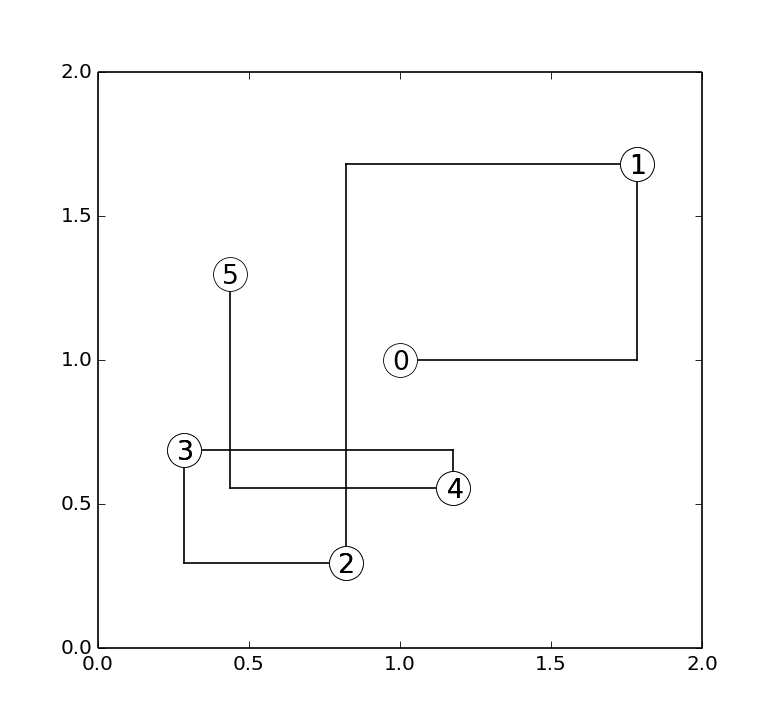
\includegraphics[width=0.48\textwidth]{toy-numbered.png}
    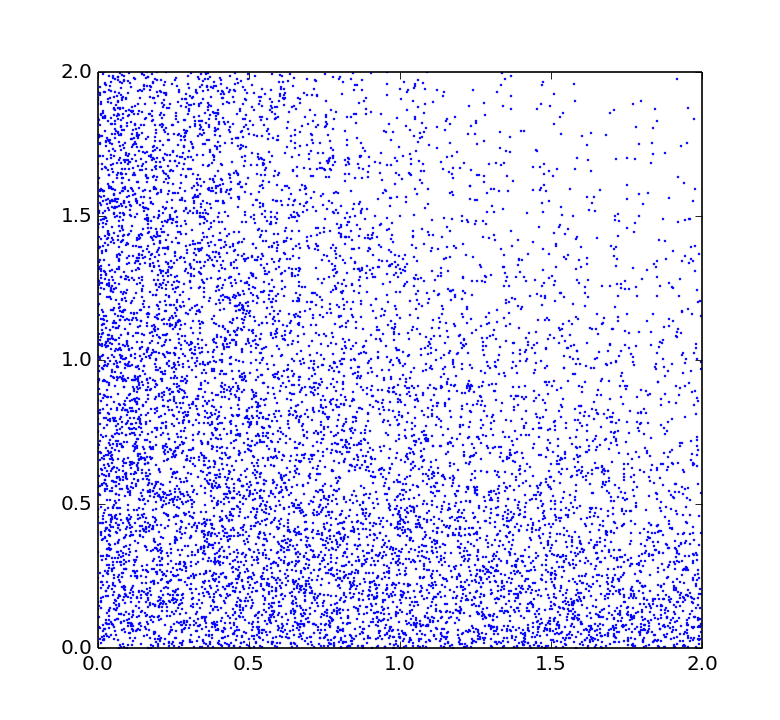
\includegraphics[width=0.48\textwidth]{toy-scatter.png}
    % Source: Original work by J. W. Miller.
  \end{center}
  \caption{(Left) Schematic representation of the first 5 Gibbs sampling iterations/sweeps/scans. (Right) Scatterplot of samples from $10^4$ Gibbs sampling iterations.}
  \label{figure:toy}
\end{figure}

So, to use Gibbs sampling, denoting $S=(0,c)$ for brevity,
\begin{enumerate}
    \item[0.] Initialize $x_0,y_0\in S$.
    \item[1.] Sample $x_1\sim \TExp(y_0,S)$, then sample $y_1\sim \TExp(x_1,S).$
    \item[2.] Sample $x_2\sim \TExp(y_1,S)$, then sample $y_2\sim \TExp(x_2,S).$\\
        $\vdots$
    \item[$N$.] Sample $x_N\sim \TExp(y_{N-1},S)$, then sample $y_N\sim \TExp(x_N,S).$
\end{enumerate}
Figure \ref{figure:toy} demonstrates the algorithm, with $c = 2$ and initial point $(x_0, y_0) = (1, 1)$.


\subsection{Example: Normal with semi-conjugate prior}
\label{section:normal}

In Chapter 4, we considered a conjugate prior for the mean $\mu$ and precision $\lambda$ of a univariate normal distribution, $\N(\mu,\lambda^{-1})$, in which the variance of $\mu|\lambda$ depended on $\lambda$. However, it is often more realistic to use independent priors on $\mu$ and $\lambda$, since we often don't expect the mean to be informative about the precision, or vice versa. In particular, consider the prior in which we take
\begin{align*}
& \bm\mu \sim \N(\mu_0,\lambda_0^{-1})\\
& \bm\lambda \sim \Ga(a,b)
\end{align*}
independently, and suppose $X_1,\ldots,X_n|\mu,\lambda\,\iid \N(\mu,\lambda^{-1})$ as usual. Unfortunately, this is not a conjugate prior. Nonetheless, it is \term{semi-conjugate} in the sense that the prior on $\mu$ is conjugate for each fixed value of $\lambda$, and the prior on $\lambda$ is conjugate for each fixed value of $\mu$. From our study of the Normal--Normal model, we know that for any fixed value of $\lambda$,
$$\bm\mu|\lambda,x_{1:n}\, \sim \,\N(M_\lambda,L_\lambda^{-1})$$
i.e., $p(\mu|\lambda,x_{1:n}) =\N(\mu\mid M_\lambda,L_\lambda^{-1})$, where $L_\lambda =\lambda_0+ n\lambda$ and
$$M_\lambda =\frac{\lambda_0\mu_0+\lambda\sum_{i = 1}^n x_i}{\lambda_0+ n\lambda}.$$
Meanwhile, for any fixed value of $\mu$, it is straightforward to derive (see Appendix) that
\begin{align}\label{equation:lambda-semi-conjugate}
\bm\lambda|\mu, x_{1:n}\,\sim\,\Ga(A_\mu, B_\mu)
\end{align}
where $A_\mu = a + n/2$ and
$$ B_\mu = b +\tfrac{1}{2}\textstyle\sum (x_i -\mu)^2 = n\hat\sigma^2 + n (\bar x-\mu)^2$$
where $\hat\sigma^2 = \frac{1}{n}\sum (x_i -\bar x)^2$. 

So, to implement Gibbs sampling in this example, each iteration would consist of sampling
\begin{align*}
    & \bm\mu|\lambda,x_{1:n}\, \sim \,\N(M_\lambda,L_\lambda^{-1})\\
    & \bm\lambda|\mu, x_{1:n}\,\sim\,\Ga(A_\mu, B_\mu).
\end{align*}


\subsection{Example: Pareto model}

Distributions of sizes and frequencies often tend to follow a ``power law'' distribution. Here are a few examples of data which have been claimed to follow this type of distribution:
\begin{itemize}
    \item wealth of individuals
    \item size of oil reserves
    \item size of cities
    \item word frequency
    \item returns on stocks
    \item size of meteorites
\end{itemize}
The Pareto distribution with shape $\alpha>0$ and scale $c >0$ has p.d.f.\
$$ \Pareto(x|\alpha,c) = \frac{\alpha c^\alpha}{x^{\alpha+1}}\I(x>c)\propto \frac{1}{x^{\alpha+1}}\I(x>c).$$
This is referred to as a power law distribution, because the p.d.f.\ is proportional to $x$ raised to a power.
Notice that $c$ is a lower bound on the observed values.
In this example, we'll see how Gibbs sampling can be used to perform inference for $\alpha$ and $c$. 

\begin{table}
\small
\centering
\begin{tabular}{clr}
Rank & City & Population \\
\hline
1  &  Charlotte   &  731424 \\
2  &  Raleigh   &  403892 \\
3  &  Greensboro   &  269666 \\
4  &  Durham   &  228330 \\
5  &  Winston-Salem   &  229618 \\
6  &  Fayetteville   &  200564 \\
7  &  Cary  &  135234 \\
8  &  Wilmington   &  106476 \\
9  &  High Point  &  104371 \\
10  &  Greenville   &  84554 \\
11  &  Asheville   &  85712 \\
12  &  Concord   &  79066 \\
13  &  Gastonia   &  71741 \\
14  &  Jacksonville   &  70145 \\
15  &  Chapel Hill  &  57233 \\
16  &  Rocky Mount  &  57477 \\
17  &  Burlington  &  49963 \\
18  &  Huntersville  &  46773 \\
19  &  Wilson   &  49167 \\
20  &  Kannapolis  &  42625 \\
21  &  Apex  &  37476 \\
22  &  Hickory  &  40010 \\
23  &  Goldsboro   &  36437 \\
24  &  Indian Trail  &  33518 \\
25  &  Mooresville  &  32711 \\
\hline
\end{tabular}
\quad
\begin{tabular}{clr}
 & & \\
\hline
26  &  Wake Forest  &  30117 \\
27  &  Monroe   &  32797 \\
28  &  Salisbury   &  33622 \\
29  &  New Bern   &  29524 \\
30  &  Sanford   &  28094 \\
31  &  Matthews  &  27198 \\
32  &  Holly Springs  &  24661 \\
33  &  Thomasville  &  26757 \\
34  &  Cornelius  &  24866 \\
35  &  Garner  &  25745 \\
36  &  Asheboro   &  25012 \\
37  &  Statesville   &  24532 \\
38  &  Mint Hill  &  22722 \\
39  &  Kernersville  &  23123 \\
40  &  Morrisville  &  18576 \\
41  &  Lumberton   &  21542 \\
42  &  Kinston   &  21677 \\
43  &  Fuquay-Varina  &  17937 \\
44  &  Havelock  &  20735 \\
45  &  Carrboro  &  19582 \\
46  &  Shelby   &  20323 \\
47  &  Clemmons  &  18627 \\
48  &  Lexington   &  18931 \\
49  &  Elizabeth City   &  18683 \\
50  &  Boone   &  17122 \\
\hline
\end{tabular}
\vspace{1em}
\caption{Populations of the 50 largest cities in the state of North Carolina, USA.}
\label{table:cities}
\end{table}


Table \ref{table:cities} shows the populations of the 50 largest cities in the state of North Carolina, according to the 2010 census.\footnote{\url{http://en.wikipedia.org/wiki/List_of_municipalities_in_North_Carolina}} The Pareto distribution is often a good model for this type of data.

\subsubsection{Model}
Let's use a Pareto model for this population data:
$$X_1,\ldots,X_n|\alpha,c\, \iid \, \Pareto(\alpha,c)$$
where $X_i$ is the population of city $i$. 
\begin{quote}
\it
\begin{itemize}
\item[Reader:] Now hold on just one second. You're going to treat the 50 largest cities as a random sample? That seems fishy.
\item[Author:] Why?
\item[Reader:] Well, clearly there is selection bias here, because you are only looking at the largest cities.
\item[Author:] Good grief, you're right! Hmm, let's see\dots
\item[Reader:] Oh, wait---it doesn't matter!
\item[Author:] Huh, why?
\item[Reader:] Because using only the largest cities is essentially like ``rejecting'' all the cities below some cutoff point $c$, and by the rejection principle, the remaining samples are distributed according to the conditional distribution given $x>c$. And if the original data was $\Pareto(x|\alpha,c_0)$ for some $c_0<c$, then the conditional distribution given $x>c$ is $\Pareto(x|\alpha,c)$, because
$$ \Pareto(x|\alpha,c_0)\I(x>c)\propto 
%\frac{1}{x^{\alpha+1}}\I(x>c_0)\I(x>c)=\frac{1}{x^{\alpha+1}}\I(x>c) \propto
\Pareto(x|\alpha,c). $$
\item[Author:] Oh, cool! So, our inferences regarding $\alpha$ will be valid, but $c$ is essentially just determining this cutoff point.
\item[Reader:] Right.  OK, good.
\end{itemize}
\end{quote}
In this example, the parameters have the following interpretation:
\begin{itemize}
\item $\alpha$ tells us the scaling relationship between the size of cities and their probability of occurring. For instance, if $\alpha = 1$
    then the density looks like $1/x^{\alpha +1} = 1/x^2$, so cities with 10,000--20,000 inhabitants occur roughly $10^{\alpha+1} = 100$
    times as frequently as cities with 100,000--110,000 inhabitants (or $10^{\alpha +1}/10 = 10$ times as frequently as cities with
    100,000--200,000 inhabitants).
\item $c$ represents the cutoff point---any cities smaller than this were not included in the dataset.
\end{itemize}
To keep things as simple as possible, let's use an (improper) flat prior:
$$p(\alpha,c) \propto \I(\alpha,c>0).$$
An \term{improper prior} is a nonnegative function of the parameters which integrates to infinity, so it can't really be considered to define a prior distribution. But, we can still plug it into Bayes' formula, and often (but not always!)\ the resulting ``posterior'' will be proper---in other words, the likelihood times the prior integrates to a finite value, and so this ``posterior'' is a well-defined a probability distribution. It is important that the ``posterior'' be proper, since otherwise the whole Bayesian framework breaks down. Improper priors are often used in an attempt to make a prior as \term{non-informative} as possible, in other words, to represent as little prior knowledge as possible. They are sometimes also mathematically convenient.

\subsubsection{Posterior}
So, plugging these into Bayes' theorem, we \textit{define} the posterior to be proportional to the likelihood times the prior:
\begin{align}
    p(\alpha,c|x_{1:n}) & \overset{\text{def}}{\underset{\alpha,c}{\propto}} p(x_{1:n}|\alpha,c)p(\alpha,c)\notag\\ 
    &\underset{\alpha,c}{\propto}\I(\alpha,c>0)\prod_{i=1}^n \frac{\alpha c^\alpha}{x_i^{\alpha+1}}\I(x_i>c) \notag\\
    & = \frac{\alpha^n c^{n\alpha}}{(\prod x_i)^{\alpha+1}} \I(c<x_*)\I(\alpha,c>0)\label{equation:Pareto-posterior}
                        % & = \alpha^n \Big(\prod_{i=1}^n c/x_i\Big)^\alpha \I(c<x_*)
\end{align}
where $x_* = \min\{x_1,\ldots,x_n\}$. As a joint distribution on $(\alpha,c)$, this does not seem to have a recognizable form, and it is not clear how we might sample from it directly. Let's try Gibbs sampling! To use Gibbs, we need to be able to sample $\alpha|c,x_{1:n}$ and $c|\alpha,x_{1:n}$. By Equation \ref{equation:Pareto-posterior}, we find that
\begin{align*}
p(\alpha|c,x_{1:n})&\underset{\alpha}{\propto}p(\alpha,c|x_{1:n})
\underset{\alpha}{\propto} \frac{\alpha^n c^{n\alpha}}{(\prod x_i)^\alpha}\I(\alpha>0) \\
&= \alpha^n\exp\big(-\alpha(\textstyle\sum\log x_i - n\log c)\big)\I(\alpha>0) \\
&\underset{\alpha}{\propto} \Ga\big(\alpha\,\big\vert\, n+1,\,\textstyle\sum\log x_i - n\log c\big),
\end{align*}
and
\begin{align*}
p(c|\alpha, x_{1:n})\underset{c}{\propto}p(\alpha,c|x_{1:n})
\underset{c}{\propto} c^{n\alpha}\I(0<c<x_*).
\end{align*}

\begin{quote}
\it
\begin{itemize}
\item[Reader:] I don't recognize the form of this distribution on $c$.
\item[Author:] Me neither, but it looks nice and simple!
\item[Reader:] Totally. It should be a piece of cake to compute the normalizing constant.
\item[Author:] Yep, and I bet the c.d.f.\ will be simple enough that we can use the inverse c.d.f.\ method to sample from it.
\item[Reader:] Let's try it.
% Ooh, what should we call it? 
% \item[Author:] It's probably already got a name, we just don't know what it is.
% \item[Reader:] So what? Let's call it the 
\end{itemize}
\end{quote}

\subsubsection{Sampling $c$ using the inverse c.d.f.\ technique}
For $a>0$ and $b>0$, define the distribution $\Mono(a,b)$ (for monomial) with p.d.f.
$$ \Mono(x|a,b)\propto x^{a-1}\I(0<x<b). $$
Since $\int_0^b x^{a -1}d x = b^a/a$, we have
$$ \Mono(x|a,b) =\frac{a}{b^a}x^{a-1}\I(0<x<b), $$
and for $0<x<b$, the c.d.f.\ is
$$ F(x|a,b) =\int_0^x \Mono(y|a,b)d y = \frac{a}{b^a}\frac{x^a}{a} = \frac{x^a}{b^a}. $$
To use the inverse c.d.f.\ technique, we solve for the inverse of $F$ on $0<x<b$:
\begin{align*}
u &= \frac{x^a}{b^a} \\
b^a u &= x^a \\ 
b u^{1/a} &= x 
\end{align*}
and thus, we can sample from $\Mono(a,b)$ by drawing $U\sim \Uniform(0,1)$ and setting $X=b U^{1/a}$.
(By the way, it turns out that this is an inverse of the Pareto distribution, in the sense that if $X\sim\Pareto(\alpha,c)$ then $1/X\sim\Mono(\alpha,1/c)$, and vice versa, but for the purposes of this example, I assumed that this was not known.)

\subsubsection{Results}
So, in order to use the Gibbs sampling algorithm to sample from the posterior $p(\alpha,c|x_{1:n})$, we initialize $\alpha$ and $c$, and then alternately update them by sampling:
\begin{align*}
\alpha|c,x_{1:n} \,&\sim\, \Ga\big(n+1,\,\textstyle\sum\log x_i - n\log c\big) \\
c|\alpha,x_{1:n}\,&\sim\, \Mono(n\alpha+1,\,x_*).
\end{align*}

\begin{figure}
    \centering
    \begin{subfigure}[t]{1\textwidth}
        \centering
        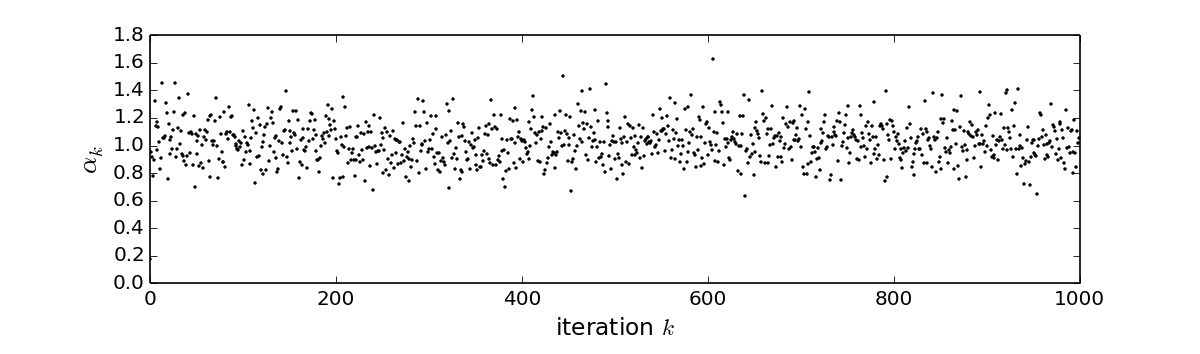
\includegraphics[trim=0 0.4cm 0 0, clip, width=0.9\textwidth]{Pareto-a_trace.png}
        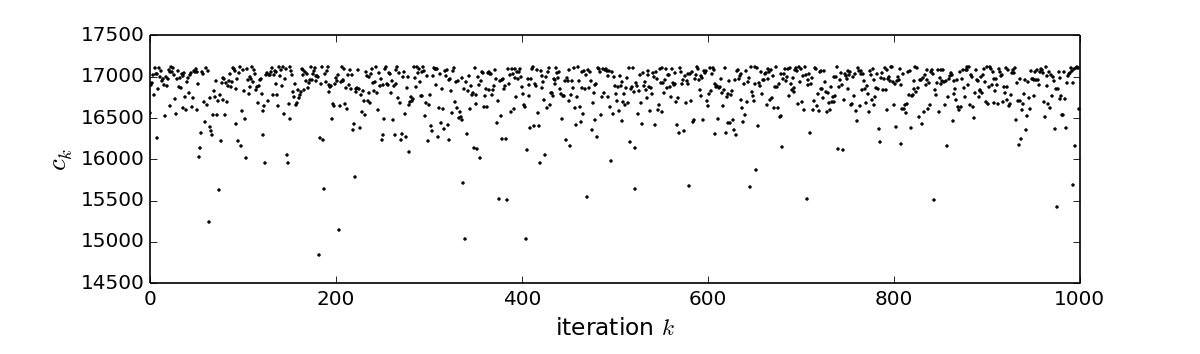
\includegraphics[trim=0 0.4cm 0 0, clip, width=0.9\textwidth]{Pareto-c_trace.png}
        % Original work by Jeffrey W. Miller
        \caption{Traceplots of $\alpha$ (top) and $c$ (bottom).}
    \end{subfigure}
    \begin{subfigure}[t]{0.49\textwidth}
        \centering
        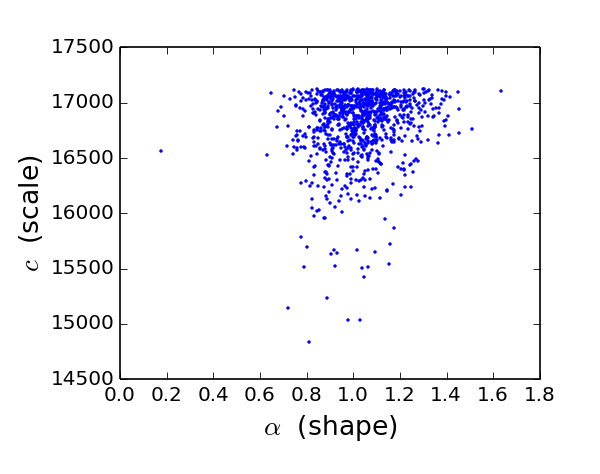
\includegraphics[trim=0 0.6cm 0 0, clip, width=1\textwidth]{Pareto-scatterplot.png}
        % Original work by Jeffrey W. Miller
        \caption{Scatterplot of samples.}
    \end{subfigure}%
    ~ 
    \begin{subfigure}[t]{0.49\textwidth}
        \centering
        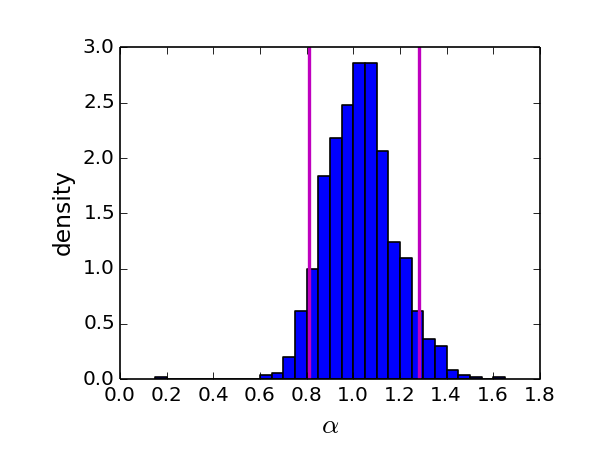
\includegraphics[trim=0 0.6cm 0 0, clip, width=1\textwidth]{Pareto-a_density.png}
        % Original work by Jeffrey W. Miller
        \caption{Estimated density of $\alpha|x_{1:n}$.}
    \end{subfigure}
    \begin{subfigure}[t]{0.49\textwidth}
        \centering
        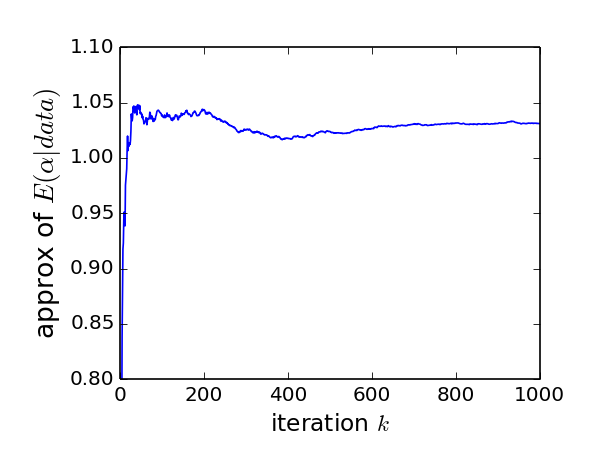
\includegraphics[trim=0 0.6cm 0 0, clip, width=1\textwidth]{Pareto-a_means.png}
        % Original work by Jeffrey W. Miller
        \caption{$\frac{1}{k}\sum_{i = 1}^k \alpha_i$ for $k=1,\ldots,N$.}
    \end{subfigure}%
    ~ 
    \begin{subfigure}[t]{0.49\textwidth}
        \centering
        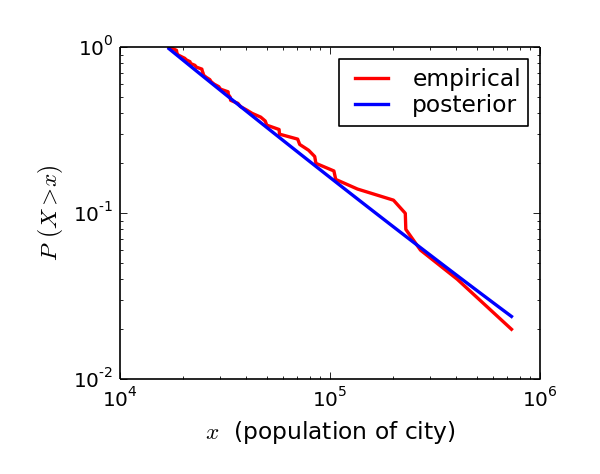
\includegraphics[trim=0 0.6cm 0 0, clip, width=1\textwidth]{Pareto-survival-function.png}
        % Original work by Jeffrey W. Miller
        \caption{Empirical vs posterior survival function.}
    \end{subfigure}
    \vspace{.5em}
    \caption{Results from the power law example.}
    \label{figure:Pareto}
\end{figure}

Initializing at $\alpha = 1$ and $c = 100$, we run the Gibbs sampler for $N = 10^3$ iterations on the 50 data points from Table \ref{table:cities}, giving us a sequence of samples
$$ (\alpha_1,c_1),\ldots,(\alpha_N,c_N). $$
Figure \ref{figure:Pareto} shows various ways of viewing the results. 
\begin{itemize}
\item[(a)] \textbf{Traceplots}. A traceplot simply shows the sequence of samples, for instance $\alpha_1,\ldots,\alpha_N$, or $c_1,\ldots, c_N$. Traceplots are a simple but very useful way to visualize how the sampler is behaving. The traceplots in Figure \ref{figure:Pareto}(a) look very healthy---the sampler doesn't appear to be getting stuck anywhere.
\item[(b)] \textbf{Scatterplot}. The scatterplot in panel (b) shows us what the posterior distribution $p(\alpha, c|x_{1:n})$ looks like. The smallest city in our data set is Boone, with a population of 17,122, and the posterior on $c$ is quite concentrated just under this value, which makes sense since $c$ represents the cutoff point in the sampling process.
\item[(c)] \textbf{Estimated density}. We are primarily interested in the posterior on $\alpha$, since it tells us the scaling relationship between the size of cities and their probability of occurring. By making a histogram of the samples $\alpha_1,\ldots,\alpha_N$, we can estimate the posterior density $p(\alpha|x_{1:n})$. The two vertical lines indicate the lower $\ell$ and upper $u$ boundaries of an (approximate) 90\% credible interval $[\ell,u]$---that is, an interval that contains 90\% of the posterior probability:
$$\Pr\big(\bm\alpha\in [\ell, u] \big\vert x_{1:n}\big) = 0.9. $$
The interval shown here is approximate since it's based on the samples. 
This can be computed from the samples by sorting them $\alpha_{(1)}\leq \cdots\leq\alpha_{(N)}$ and setting
$$\ell = \alpha_{(\lfloor 0.05 N\rfloor)}  \qquad u = \alpha_{(\lceil 0.95 N\rceil)} $$
where $\lfloor x\rfloor$ and $\lceil x\rceil$ are the floor and ceiling functions, respectively.
\item[(d)] \textbf{Running averages}. Panel (d) shows the running average $\frac{1}{k}\sum_{i = 1}^k\alpha_i$ for $k = 1,\ldots,N$. In addition to traceplots, running averages such as this are a useful heuristic for visually assessing the convergence of the Markov chain. The running average shown in this example still seems to be meandering about a bit, suggesting that the sampler needs to be run longer (but this would depend on the level of accuracy desired).
\item[(e)] Panel (e) is particular to this example. Power law distributions are often displayed by plotting their survival function $S(x)$---that is, one minus the c.d.f., $S(x) = \Pr(X>x) = 1-\Pr(X\leq x)$---on a log-log plot, since $S(x) = (c/x)^\alpha$ for the $\Pareto(\alpha,c)$ distribution and on a log-log plot this appears as a line with slope $-\alpha$. The posterior survival function (or more precisely, the posterior predictive survival function), is $S(x|x_{1:n}) = \Pr(X_{n+1}>x\mid x_{1:n})$. Figure \ref{figure:Pareto}(e) shows an empirical estimate of the survival function (based on the empirical c.d.f., $\hat F(x) = \frac{1}{n}\sum_{i = 1}^n \I(x\geq x_i)$) along with the posterior survival function, approximated by
\begin{align*}
S(x|x_{1:n}) &= \Pr(X_{n+1}>x\mid x_{1:n}) = \int \Pr(X_{n+1}>x\mid \alpha,c) p(\alpha,c|x_{1:n})d\alpha d c\\
&\approx\frac{1}{N}\sum_{i = 1}^N \Pr(X_{n+1}>x\mid \alpha_i,c_i)
=\frac{1}{N}\sum_{i = 1}^N (c_i/x)^{\alpha_i}.
\end{align*}
This is computed for each $x$ in a grid of values.
\end{itemize}
It is important to note that even when heuristics like traceplots and running averages appear to indicate that all is well, it is possible that things are going horribly wrong. For instance, it is not uncommon for there to be multiple modes, and for the sampler to get stuck in one of them for many iterations.











\section{Gibbs sampling with more than two variables}

In Section \ref{section:Gibbs-sampling-with-two-variables}, we saw how to use Gibbs sampling for distributions with two variables, e.g., $p(x,y)$. The generalization to more than two variables is completely straightforward---roughly speaking, we cycle through the variables, sampling each from its conditional distributional given all the rest.

For instance, for a distribution with three random variables, say, $p(x,y,z)$, we set $x$, $y$, and $z$ to some initial values, and then sample $x|y,z$, then $y|x,z$, then $z|x,y$, then $x|y,z$, and so on. More precisely,
\begin{enumerate}
\item[0.] Set $(x_0,y_0,z_0)$ to some starting value.
\item[1.] Sample $x_1\sim p(x|y_0,z_0)$. \\
          Sample $y_1\sim p(y|x_1,z_0)$. \\
          Sample $z_1\sim p(z|x_1,y_1)$. \\
\item[2.] Sample $x_2\sim p(x|y_1,z_1)$. \\
          Sample $y_2\sim p(y|x_2,z_1)$. \\
          Sample $z_2\sim p(z|x_2,y_2)$. \\
        $\vdots$
\end{enumerate}

In general, for distribution with $d$ random variables, say, $p(v^1,\ldots,v^d)$, at each iteration of the algorithm, we sample from
\begin{align*}
v^1&\mid v^2,v^3,\ldots,v^d\\
v^2&\mid v^1,v^3,\ldots,v^d\\
&\vdots\\
v^d&\mid v^1,v^2,\ldots,v^{d-1}
\end{align*}
always using the most recent values of all the other variables. The conditional distribution of a variable given all of the others is sometimes referred to as the \term{full conditional} in this context, and for brevity this is sometimes denoted $v^i|\cdots$.




\subsection{Example: Censored data}
In many real-world data sets, some of the data is either missing altogether or is partially obscured. Gibbs sampling provides a method for dealing with these situations in a completely coherent Bayesian way, by sampling these missing variables along with the parameters. This also provides information about the values of the missing/obscured data.

One way in which data can be partially obscured is by \term{censoring}, which means that we know a data point lies in some particular interval, but we don't get to observe it exactly. Censored data occurs very frequently in medical research such as clinical trials (since for instance, the researchers may lose contact with some of the patients), and also in engineering (since some measurements may exceed the lower or upper limits of the instrument being used).

To illustrate, suppose researchers are studying the length of life (lifetime) following a particular medical intervention, such as a new surgical treatment for heart disease, and in a study of 12 patients, the number of years before death for each is
$$3.4, 2.9, 1.2+, 1.4, 3.2, 1.8, 4.6, 1.7+, 2.0+, 1.4+, 2.8, 0.6+$$
where $x+$ indicates that the patient was alive after $x$ years, but the researchers lost contact with the patient at that point. (Of
course, there will always also be a control group, but let's focus on one group to keep things simple.) Consider the following model:
\begin{align*}
    &\btheta\sim \Ga(a, b)\\
    &Z_1,\ldots,Z_n|\theta\,\iid\,\Ga(r,\theta)\\
    &X_i = \branch{Z_i}{Z_i\leq c_i}{\ast}{Z_i > c_i.}
\end{align*}
where $a$, $b$, and $r$ are known, and $\ast$ is a special value to indicate that censoring has occurred.  The interpretation is:
\begin{itemize}
    \item $\theta$ is the parameter of interest---the rate parameter for the lifetime distribution.
    \item $Z_i$ is the lifetime for patient $i$, however, this is not directly observed.
    \item $c_i$ is the censoring time for patient $i$, which is fixed, but known only if censoring occurs.
    \item $X_i$ is the observation---if the lifetime is less than $c_i$ then we get to observe it ($X_i = Z_i$), otherwise
        all we know is the lifetime is greater than $c_i$ ($X_i = \ast$).
\end{itemize}

\subsubsection{The posterior is complicated}
Unfortunately, the posterior $p(\theta|x_{1:n}) \propto p(x_{1:n}|\theta)p(\theta)$ does not reduce to a simple form that we can easily work with. The reason is that the likelihood $p(x_{1:n}|\theta)$ involves the distribution of the observations $x_i$ given $\theta$, integrating out the $z_i$'s, and in the case of censored observations $x_i=\ast$, this is
$$p(x_i|\theta) = \Pr(X_i = \ast \mid \theta) = \Pr(Z_i>c\mid \theta),$$
which is one minus the $\Ga(r,\theta)$ c.d.f., a rather complicated function of $\theta$.

Also, $p(z_{1:n}|x_{1:n})$ (the posterior on the $z_i$'s, with $\theta$ integrated out) looks a bit nasty as well, and it's not immediately clear to me how one would sample from it.


\subsubsection{Gibbs sampling approach}
Meanwhile, the Gibbs sampling approach is a cinch. To sample from $p(\theta,z_{1:n}|x_{1:n})$, we cycle through each of the full conditional distributions,
\begin{align*}
\theta &\mid z_{1:n}, x_{1:n}\\
z_1 &\mid \theta, z_{2:n}, x_{1:n}\\
z_2 &\mid \theta, z_1,z_{3:n}, x_{1:n}\\
\vdots\\
z_n &\mid \theta, z_{1:n-1}, x_{1:n}
\end{align*}
sampling from each in turn, always conditioning on the most recent values of the other variables.
The full conditionals are easy to calculate:
\begin{itemize}
\item ($\theta|\cdots$) Since $\theta \perp x_{1:n}\mid z_{1:n}$ (i.e., $\theta$ is conditionally independent of $x_{1:n}$ given $z_{1:n}$),
$$p(\theta|\cdots) = p(\theta|z_{1:n},x_{1:n}) = p(\theta|z_{1:n}) = \Ga\big(\theta\,\big\vert\, a+nr,\, b+\textstyle\sum_{i=1}^n z_i\big)$$
using the fact that the prior on $\theta$ is conjugate. (See Exercise 3 of Chapter 3.)
\item ($z_i|\cdots$) If $x_i\neq \ast$ then $z_i$ is forced to be equal to $x_i$. Otherwise,
\begin{align*}
p(z_i|\cdots) &= p(z_i|\theta,z_{(1:n) - i}, x_{1:n}) = p(z_i|\theta,x_i) \\
&\underset{z_i}{\propto} p(x_i,z_i|\theta) = p(x_i|z_i) p(z_i|\theta)\\
& =\I(z_i>c_i)\Ga(z_i\mid r,\theta)\\
& \underset{z_i}{\propto} \TGamma(z_i\mid r,\theta,(c_i,\infty))
\end{align*}
where $\TGamma(z_i\mid r,\theta,S)$ is the truncated Gamma distribution---that is, the distribution of a $\Ga(r,\theta)$ random variable conditioned on being in the set $S$.
\end{itemize}
We can sample from $\TGamma(r,\theta,(c,\infty))$ with the same approach we used for the truncated exponential in Section \ref{section:toy}: if $F(x|r,\theta)$ denotes the $\Ga(r,\theta)$ c.d.f., then to draw a sample $Z\sim\TGamma(r,\theta,(c,\infty))$,
\begin{enumerate}
\item sample $U\sim\Uniform(F(c|r,\theta),1)$, and
\item set $Z = F^{-1}(U|r,\theta)$.
\end{enumerate}

\begin{figure}
    \centering
    \begin{subfigure}[t]{1\textwidth}
        \centering
        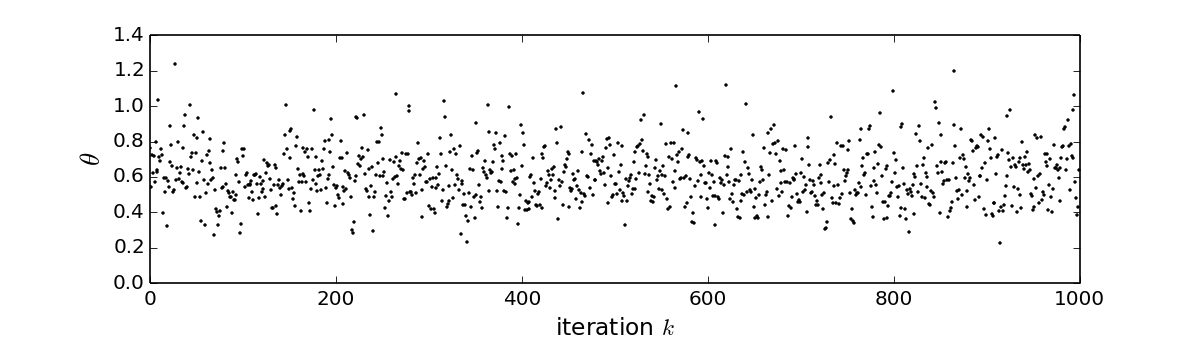
\includegraphics[trim=0 0.4cm 0 0, clip, width=0.9\textwidth]{censored-theta_trace.png}
        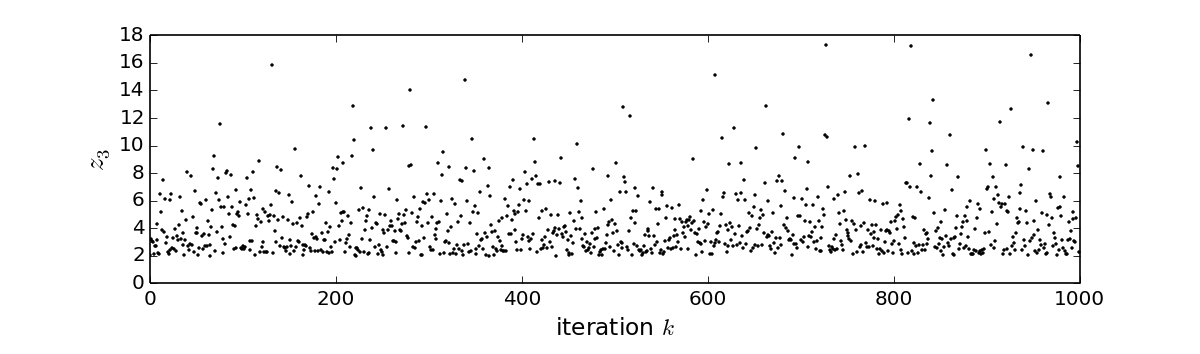
\includegraphics[trim=0 0.4cm 0 0, clip, width=0.9\textwidth]{censored-z_trace.png}
        % Original work by Jeffrey W. Miller
        \caption{Traceplots of $\theta$ (top) and $z_9$ (bottom).}
    \end{subfigure}
    \begin{subfigure}[t]{1\textwidth}
        \centering
        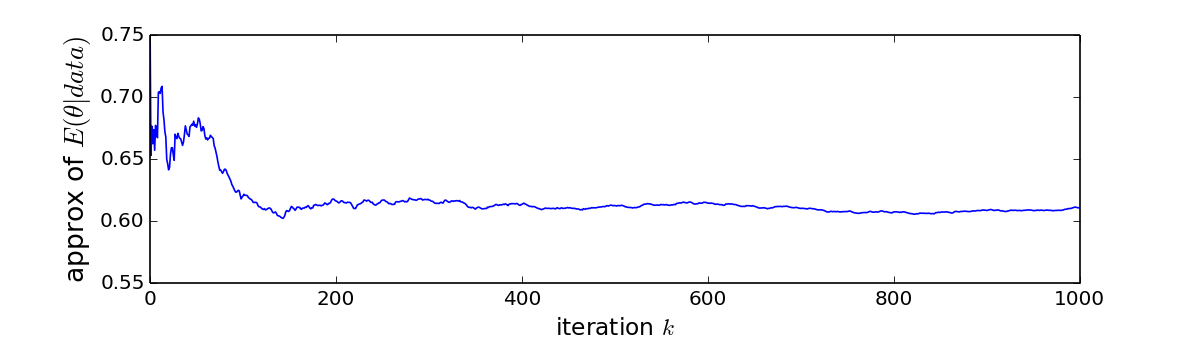
\includegraphics[trim=0 0.2cm 0 0, clip, width=0.9\textwidth]{censored-theta_means.png}
        % Original work by Jeffrey W. Miller
        \caption{Running averages $\frac{1}{k}\sum_{i = 1}^k \theta_i$ for $k=1,\ldots,N$.}
    \end{subfigure}
    \begin{subfigure}[t]{0.49\textwidth}
        \centering
        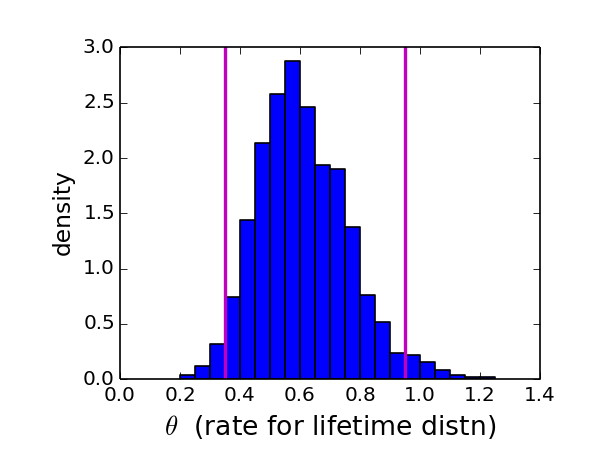
\includegraphics[trim=0 0.6cm 0 0, clip, width=1\textwidth]{censored-theta_density.png}
        % Original work by Jeffrey W. Miller
        \caption{Estimated density of $\theta|x_{1:n}$.}
    \end{subfigure}%
    ~ 
    \begin{subfigure}[t]{0.49\textwidth}
        \centering
        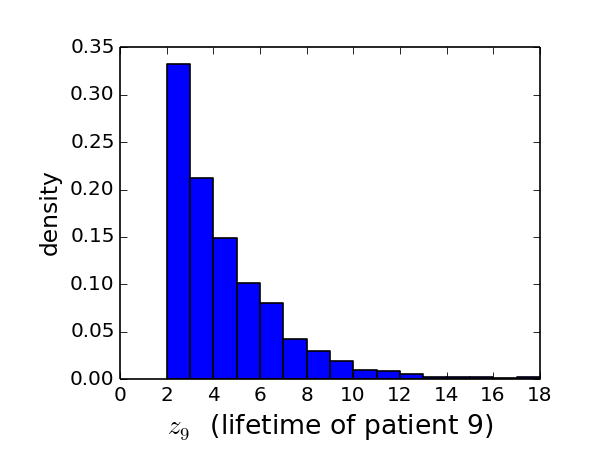
\includegraphics[trim=0 0.6cm 0 0, clip, width=1\textwidth]{censored-z_density.png}
        % Original work by Jeffrey W. Miller
        \caption{Estimated density of $z_9|x_{1:n}$.}
    \end{subfigure}
    \vspace{.5em}
    \caption{Results from the censoring example.}
    \label{figure:censored}
\end{figure}

\subsubsection{Results}

Let's suppose $a = b = 1$ and $r = 2.0$, and run the Gibbs sampler for $N = 10^3$ iterations, using initial values $\theta = 1$ and $z_i = c_i+1$ for those $i$'s that were censored.
See Figure \ref{figure:censored} for various traceplots, running averages, and estimated densities.




\subsection{Example: Hyperpriors and hierarchical models}

Gibbs sampling is spectacularly useful for models involving multiple levels, particularly when each piece of the model involves a conjugate (or at least semi-conjugate) prior. For instance, we may want to put a prior not only on the parameters, but also on the hyperparameters---that is, the parameters of the prior---this is called a \term{hyperprior}. This comes up particularly often when constructing \term{hierarchical models}, that is, models in which there is a hierarchical structure to the relationships between the data, latent variables, and parameters.

As a simple example, consider the Normal model with semi-conjugate prior from Section \ref{section:normal}. Let's put a $\Ga(r,s)$ hyperprior
on $\lambda_0$, so that the model is now:
\begin{align*}
& \bm\lambda_0 \sim \Ga(r,s)\\
& \bm\mu|\lambda_0\,\sim\,\N(\mu_0,\lambda_0^{-1})\\
& \bm\lambda \sim \Ga(a,b)\\
& X_1,\ldots,X_n|\lambda_0,\mu,\lambda\,\sim\,\N(\mu,\lambda^{-1}).
\end{align*}
You might recognize that this is equivalent to putting a $t$-distribution prior on $\mu$. Since the $t$-distribution is not a conjugate prior
for the mean of Normally-distributed data, we would not be able to sample directly from $\mu|\lambda,x_{1:n}$.  However, we \textit{can}
easily sample from $\mu|\lambda_0,\lambda,x_{1:n}$, and this is what we need for Gibbs sampling.

\subsubsection{Gibbs sampler}
\begin{itemize}
    \item ($\lambda_0|\cdots$) Since $\lambda_0$ is conditionally independent of everything else given $\mu$, this is exactly the same as
        the posterior on the precision in a semi-conjugate Normal model with one datapoint (namely, $\mu$). Thus,
        $$\bm\lambda_0|\mu,\lambda,x_{1:n} \,\sim\, \Ga\big(r+1/2,\,s+\tfrac{1}{2}(\mu-\mu_0)^2\big).$$
    \item ($\mu|\cdots$) Since we are conditioning on $\lambda_0$, we are just in the usual situation for the semi-conjugate Normal
        model without a hyperprior, and thus, just like in Section \ref{section:normal},
        $$\bm\mu|\lambda_0,\lambda,x_{1:n}\, \sim \,\N(M,L^{-1})$$
        where $L =\lambda_0+ n\lambda$ and $M =(\lambda_0\mu_0+\lambda\sum x_i)/(\lambda_0+ n\lambda)$.
    \item ($\lambda|\cdots$) We are again just in the usual situation for the semi-conjugate Normal, and thus
        $$\bm\lambda|\lambda_0,\mu,x_{1:n}\,\sim\,\Ga(A,B)$$
        where $A = a + n/2$ and $B = n\hat\sigma^2 + n (\bar x-\mu)^2$.
\end{itemize}
Each iteration of Gibbs sampling proceeds by sampling from each of these, in turn.

We could just as easily put (semi-)conjugate priors on $\mu_0$ and $b$ as well (specifically, a Normal prior on $\mu_0$ and a Gamma prior on
$b$), and include them as well in the Gibbs sampling algorithm.  In this simple example, these hyperpriors essentially just make the prior
less informative, however, when constructing hierarchical models involving multiple groups of datapoints, this approach can enable the
``sharing of statistical strength'' across groups---roughly, using information learned from one group to help make inferences about the
others.  
%There is almost no limit to the complexity of models that can be built in this way, and in principle, Gibbs sampling can easily be
%used to do inference on them. However, one needs to be careful that the sampler is ``mixing'' well, i.e., converging.




\subsection{Example: Data augmentation / Auxiliary variables}

A commonly-used technique for designing MCMC samplers is to use \term{data augmentation}, also known as \term{auxiliary variables}.
The idea is to introduce a new variable (or variables) $Z$ that depends on the distribution of the existing variables in such a way that the
resulting conditional distributions, with $Z$ included, are easier to sample from and/or result in better mixing (faster convergence). 
So, the $Z$'s are essentially latent/hidden variables that are introduced for the purpose of simplifying/improving the sampler.
For instance, suppose we want to sample from $p(x,y)$, but $p(x|y)$ and/or $p(y|x)$ are complicated.  If we can choose some $p(z|x,y)$ such
that $p(x|y,z)$, $p(y|x,z)$, and $p(z|x,y)$ are easy to sample from, then we can construct a Gibbs sampler to sample all three variables
$(X,Y,Z)$ from $p(x,y,z)$ and then just throw away the $Z$'s and we will have samples $(X,Y)$ from $p(x,y)$.

\begin{figure}
  \begin{center}
    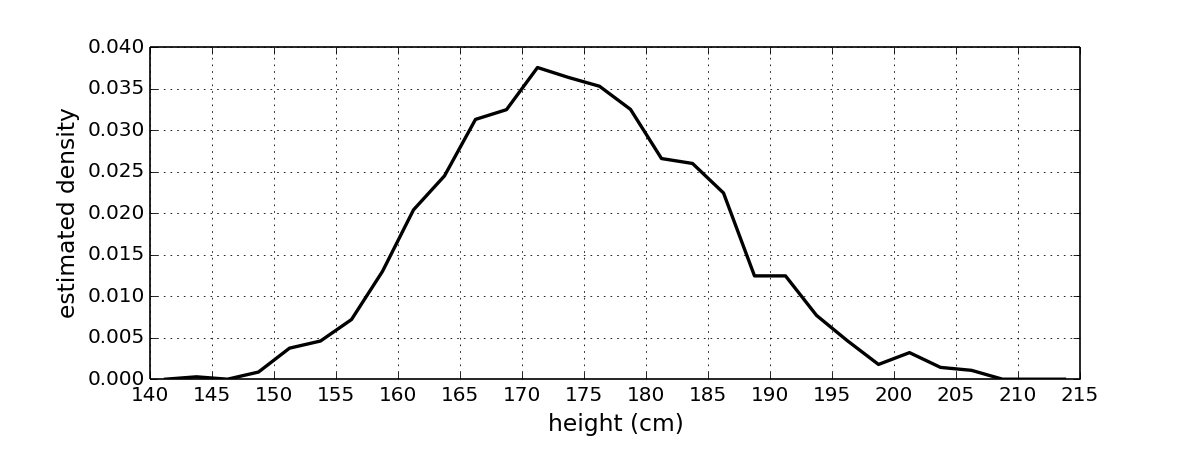
\includegraphics[width=1\textwidth]{heights-combined.png}
    % Source: Original work by J. W. Miller.
  \end{center}
  \caption{Heights of Dutch women and men, combined.}
  \label{figure:heights-combined}
\end{figure}

To illustrate, consider the data set from Chapter 4 consisting of the heights of 695 Dutch women and 562 Dutch men.  Suppose we have the list of heights, but we don't know which datapoints
are from women and which are from men.  See Figure \ref{figure:heights-combined}.
Can we still infer the distribution of female heights and male heights, e.g., the mean for males and the mean for females?  
% todo: we don't exactly do this...
Perhaps surprisingly, the answer is yes.  The reason is that this is a two-component mixture of Normals,
and there is an (essentially) unique set of mixture parameters corresponding to any such distribution.

To construct a Gibbs sampler for a mixture model such as this, it is common to introduce an auxiliary variable $Z_i$ for each datapoint,
indicating which mixture component it is drawn from. For instance, in this example, $Z_i$ would indicate whether subject $i$ is female or male.
This results in a Gibbs sampler that is quite easy to derive and implement.

\subsubsection{Two-component mixture model}
To keep things as simple as possible, let's assume that both mixture components (female and male) have the same precision
(inverse variance), say $\lambda$, and that $\lambda$ is fixed and known.  Then the usual two-component Normal mixture model is:
\begin{align*}
    & \mu_0,\mu_1 \iid \N(m,\ell^{-1})\\
    & \pi \sim \Beta(a,b)\\
    & X_1,\ldots,X_n|\mu,\pi\,\iid\,F(\mu,\pi)
\end{align*}
where $F(\mu,\pi)$ is the distribution with p.d.f. 
$$ f(x|\mu,\pi) = (1-\pi)\N(x\mid \mu_0,\lambda^{-1}) + \pi\N(x\mid \mu_1,\lambda^{-1}) $$
and $\mu=(\mu_0,\mu_1)$.

The likelihood is
\begin{align*}
    p(x_{1:n}|\mu,\pi) &= \prod_{i=1}^n f(x_i|\mu,\pi) \\
                       & = \prod_{i=1}^n \Big[ (1-\pi)\N(x_i\mid \mu_0,\lambda^{-1}) + \pi\N(x_i\mid \mu_1,\lambda^{-1}) \Big] 
\end{align*}
which is a complicated function of $\mu$ and $\pi$, making the posterior difficult to sample from directly.

\subsubsection{Allocation variables to the rescue}
We can define an equivalent model that includes latent ``allocation'' variables $Z_1,\ldots,Z_n$ to indicate which mixture component each datapoint
comes from---that is, $Z_i$ indicates whether subject $i$ is female or male.
\begin{align*}
    & \mu_0,\mu_1 \iid \N(m,\ell^{-1})\\
    & \pi \sim \Beta(a,b)\\
    & Z_1,\ldots,Z_n|\mu,\pi\,\iid\,\Bernoulli(\pi)\\
    & X_i\sim\N(\mu_{Z_i},\lambda^{-1}) \text{ independently for } i=1,\ldots,n.
\end{align*}
This is equivalent to the model above, since
\begin{align*}
    p(x_i|\mu,\pi) &= p(x|Z_i=0,\mu,\pi)\Pr(Z_i=0|\mu,\pi) 
                    + p(x|Z_i=1,\mu,\pi)\Pr(Z_i=1|\mu,\pi) \\
            &= (1-\pi)\N(x_i|\mu_0,\lambda^{-1}) + \pi\N(x_i|\mu_1,\lambda^{-1})\\
            &= f(x_i|\mu,\pi),
\end{align*}
and thus it induces the same distribution on $(x_{1:n},\mu,\pi)$. However, it is considerably easier to work with, particularly for Gibbs
sampling. 

\subsubsection{Gibbs sampling}
We derive the full conditionals. For brevity, denote $x=x_{1:n}$ and $z=z_{1:n}$.
\begin{itemize}
    \item ($\pi|\cdots$) Given $z$, $\pi$ is independent of everything else, so this reduces to a Beta--Bernoulli model, and we have
        $$ p(\pi|\mu,z,x) = p(\pi|z) =\Beta(\pi\mid a + n_1,\, b + n_0) $$
        where $n_k = \sum_{i=1}^n \I(z_i=k)$ for $k \in \{0, 1\}$.
    \item ($\mu|\cdots$) Given $z$, we know which component each datapoint comes from , so the model (conditionally on $z$) is just two
        independent Normal--Normal models, and thus (like in Section \ref{section:normal}):
        \begin{align*}
            \bm\mu_0|\mu_1,x,z,\pi\, \sim \,\N(M_0,L_0^{-1})\\
            \bm\mu_1|\mu_0,x,z,\pi\, \sim \,\N(M_1,L_1^{-1})
        \end{align*}
        where for $k\in\{0,1\}$,
        \begin{align*}
        n_k &= \sum_{i=1}^n \I(z_i=k)\\
        L_k &=\ell + n_k\lambda\\
        M_k &=\frac{\ell m + \lambda\sum_{i:z_i=k} x_i}{\ell + n_k\lambda}.
        \end{align*}
    \item ($z|\cdots$)
        \begin{align*}
            p(z|\mu,\pi,x)&\underset{z}{\propto}p(x,z,\pi,\mu)\underset{z}{\propto} p(x|z,\mu) p(z|\pi)\\
            & =\prod_{i = 1}^n \N(x_i|\mu_{z_i},\lambda^{-1})\Bernoulli(z_i|\pi)\\
            & =\prod_{i = 1}^n \Big(\pi\N(x_i|\mu_1,\lambda^{-1})\Big)^{z_i} \Big((1-\pi)\N(x_i|\mu_0,\lambda^{-1})\Big)^{1-z_i}\\
            & =\prod_{i = 1}^n \alpha_{i,1}^{z_i} \alpha_{i,0}^{1-z_i}\\
            &\underset{z}{\propto}\prod_{i = 1}^n\Bernoulli(z_i\mid \alpha_{i,1}/(\alpha_{i,0}+\alpha_{i,1}))
        \end{align*}
        where
        \begin{align*}
            \alpha_{i,0} & =(1-\pi)\N(x_i|\mu_0,\lambda^{-1})\\
            \alpha_{i,1} & =\pi\N(x_i|\mu_1,\lambda^{-1}).
        \end{align*}
\end{itemize}
As usual, each iteration of Gibbs sampling proceeds by sampling from each of these conditional distributions, in turn.


\subsubsection{Results}

\begin{figure}
    \centering
    \begin{subfigure}[t]{1\textwidth}
        \centering
        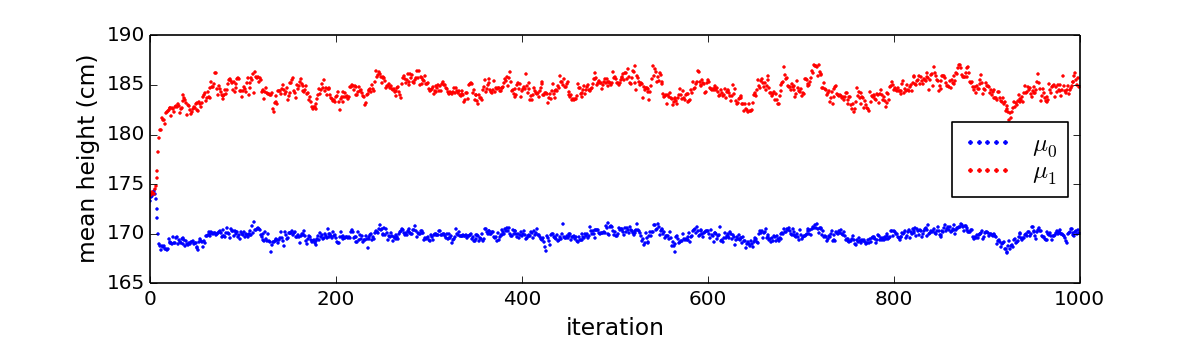
\includegraphics[trim=0 0.4cm 0 0, clip, width=1\textwidth]{mix-mu_trace-a.png}
        % Original work by Jeffrey W. Miller
        \caption{Traceplots of the component means, $\mu_0$ and $\mu_1$.}
    \end{subfigure}
    \begin{subfigure}[t]{1\textwidth}
        \centering
        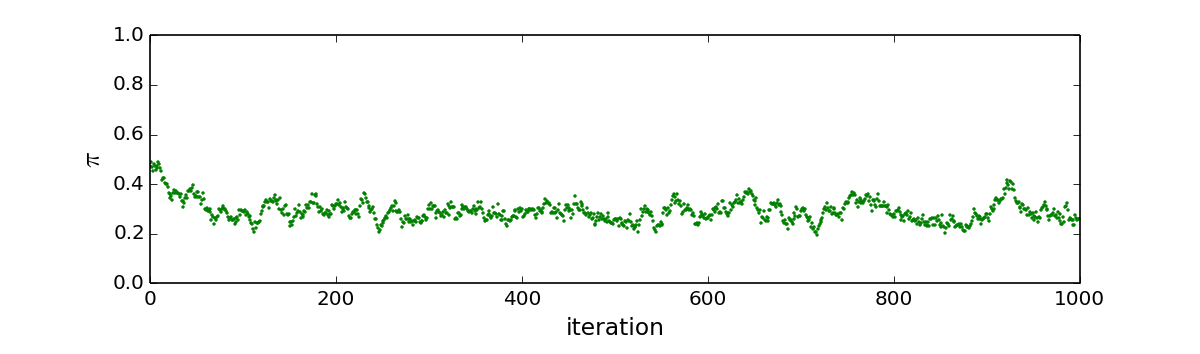
\includegraphics[trim=0 0.4cm 0 0, clip, width=1\textwidth]{mix-p_trace-a.png}
        % Original work by Jeffrey W. Miller
        \caption{Traceplot of the mixture weight, $\pi$ (prior probability that a subject comes from component 1).}
    \end{subfigure}
    \begin{subfigure}[t]{1\textwidth}
        \centering
        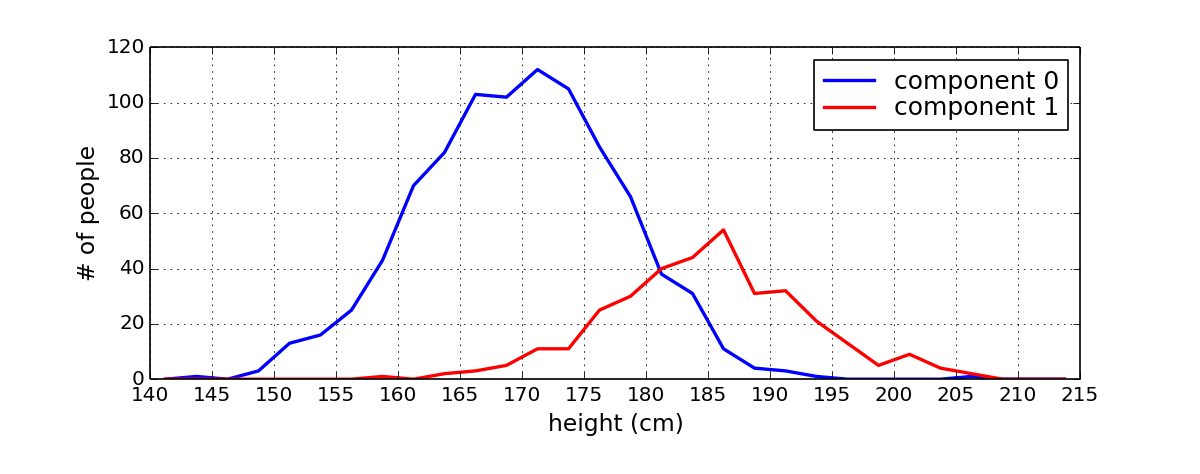
\includegraphics[trim=0 0.4cm 0 0, clip, width=1\textwidth]{mix-histograms_at_last_sample-a.png}
        % Original work by Jeffrey W. Miller
        \caption{Histograms of the heights of subjects assigned to each component, according to $z_1,\ldots,z_n$, in a typical sample.}
    \end{subfigure}
    \vspace{.5em}
    \caption{Results from one run of the mixture example.}
    \label{figure:mix}
\end{figure}

We implement this Gibbs sampler with the following parameter settings:
\begin{itemize}
\item $\lambda = 1/\sigma^2$ where $\sigma = 8$ cm ($\approx 3.1$ inches) ($\sigma$ = standard deviation of the subject heights within each component)
\item $a = 1$, $b = 1$ (Beta parameters, equivalent to prior ``sample size'' of 1 for each component)
\item $m = 175$ cm ($\approx 68.9$ inches) (mean of the prior on the component means)
\item $\ell = 1/s^2$ where $s = 15$ cm ($\approx 6$ inches) ($s$ = standard deviation of the prior on the component means)
\end{itemize}
We initialize the sampler at:
\begin{itemize}
\item $\pi = 1/2$ (equal probability for each component)
\item $z_1,\ldots,z_n$ sampled i.i.d.\ from $\Bernoulli(1/2)$ (initial assignment to components chosen uniformly at random)
\item $\mu_0 =\mu_1 = m$ (component means initialized to the mean of their prior)
\end{itemize}
Figure \ref{figure:mix} shows a few plots of the results for $N = 10^3$ iterations. (Note: This should probably be run for longer---this short run is simply for illustration purposes.) From the traceplots of $\mu_0$ and $\mu_1$, we see that one component quickly settles to have a mean of around 168--170 cm and the other to a mean of around 182--186 cm. Recalling that we are not using the true assignments of subjects to components (that is, we don't know whether they are male or female), it is interesting to note that this is fairly close to the sample averages: 168.0 cm (5 feet 6.1 inches) for females, and 181.4 cm (5 feet 11.4 inches) for males.

The traceplot of $\pi$ indicates that the sampler is exploring values of around 0.2 to 0.4---that is, the proportion of people coming from group 1 is around 0.2 to 0.4. Meanwhile, looking at the actual labels (female and male), the empirical proportion of males is $562/(695+562) \approx 0.45$. So this is slightly off. This could be due to not having enough data, and/or due to the fact that we are assuming a fixed value of $\lambda$. It would be much better, and nearly as easy, to allow components 0 and 1 to have different precisions, $\lambda_0$ and $\lambda_1$, and put Gamma priors on them.
 
As shown in the bottom plot (panel (c)), one way of visualizing the allocation/assignment variables $z_1,\ldots,z_n$ is to make histograms of the heights of the subjects assigned to each component. At a glance, this shows us where the two clusters of datapoints are, how large each cluster is, and what shape they have.


\subsubsection{A potentially serious issue: It's not mixing!}

\begin{figure}
    \centering
    \begin{subfigure}[t]{1\textwidth}
        \centering
        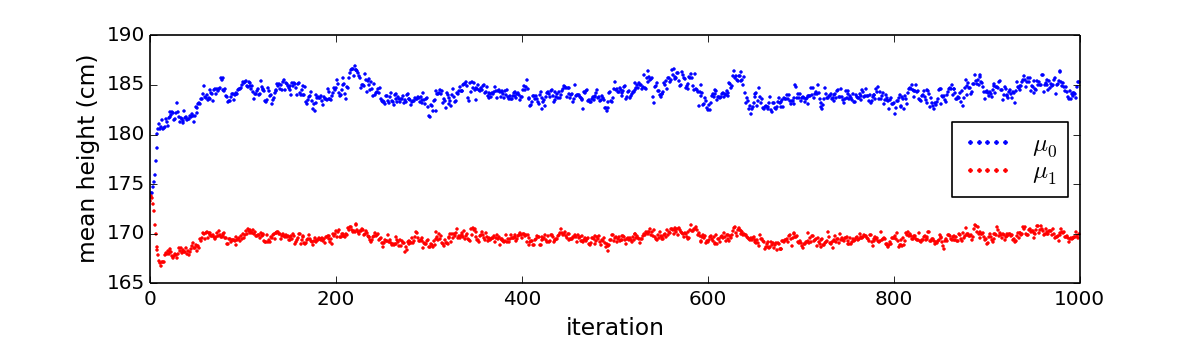
\includegraphics[trim=0 0.4cm 0 0, clip, width=1\textwidth]{mix-mu_trace-b.png}
        % Original work by Jeffrey W. Miller
        \caption{Traceplots of the component means, $\mu_0$ and $\mu_1$.}
    \end{subfigure}
    \begin{subfigure}[t]{1\textwidth}
        \centering
        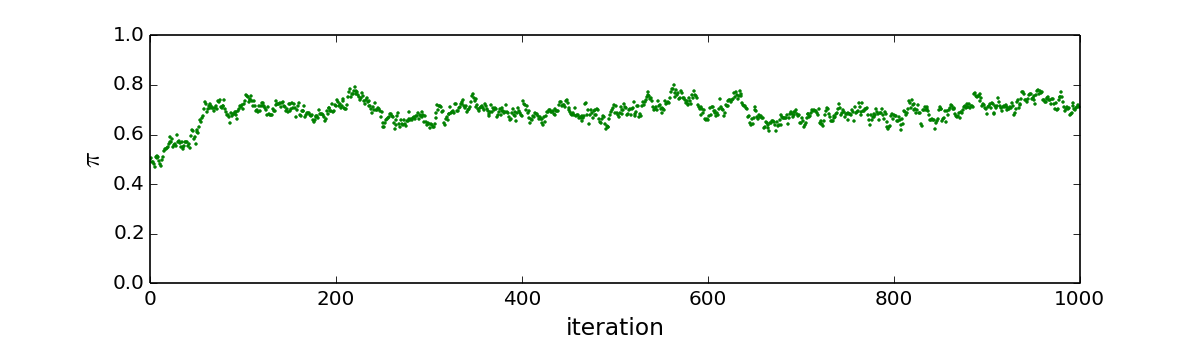
\includegraphics[trim=0 0.4cm 0 0, clip, width=1\textwidth]{mix-p_trace-b.png}
        % Original work by Jeffrey W. Miller
        \caption{Traceplot of the mixture weight, $\pi$ (prior probability that a subject comes from component 1).}
    \end{subfigure}
    \begin{subfigure}[t]{1\textwidth}
        \centering
        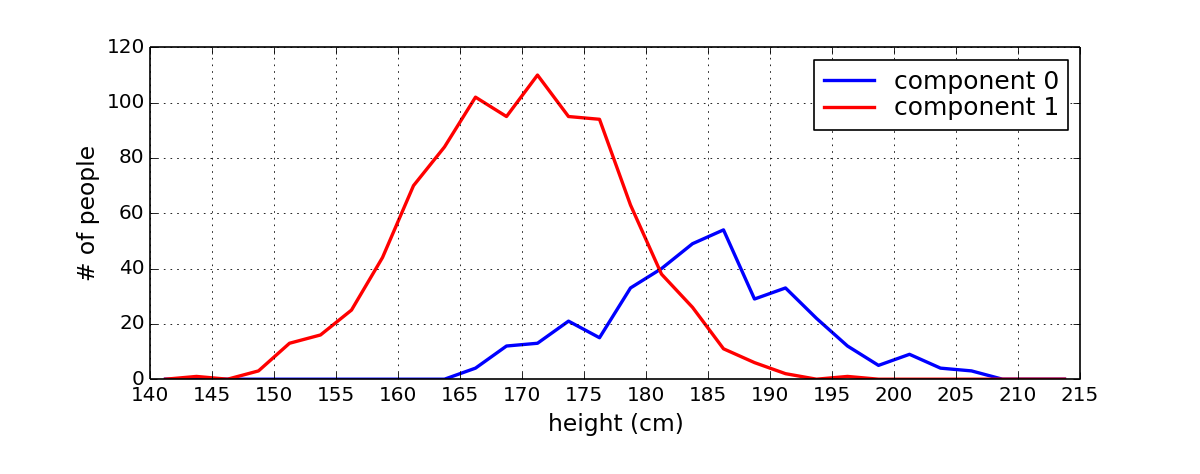
\includegraphics[trim=0 0.4cm 0 0, clip, width=1\textwidth]{mix-histograms_at_last_sample-b.png}
        % Original work by Jeffrey W. Miller
        \caption{Histograms of the heights of subjects assigned to each component, according to $z_1,\ldots,z_n$, in a typical sample.}
    \end{subfigure}
    \vspace{.5em}
    \caption{Results from another run of the mixture example.}
    \label{figure:mix-b}
\end{figure}

This example illustrates one of the big things that can go wrong with MCMC (although fortunately, in this case, the results are still valid if interpreted correctly). Why are females assigned to component 0 and males assigned to component 1? Why not the other way around? In fact, the model is symmetric with respect to the two components, and thus the posterior is also symmetric. If we run the sampler multiple times (starting from the same initial values), sometimes it will settle on females as 0 and males as 1, and sometimes on females as 1 and males as 0 --- see Figure \ref{figure:mix-b}. Roughly speaking, the posterior has two modes. If the sampler were behaving properly, it would move back and forth between these two modes, but it doesn't---it gets stuck in one and stays there.

This is a very common problem with mixture models. Fortunately, however, in the case of mixture models, the results are still valid if we interpret them correctly. Specifically, our inferences will be valid as long as we only consider quantities that are invariant with respect to permutations of the components.


% However, in a certain sense, this type of mixture sampler usually has extremely poor performance, as we will see below. 
% This illustrates one of the big issues that can arise with MCMC---when there are multiple modes separated by a relatively large region of
% small probability, the sampler can get stuck in one of these modes.  In the case of mixtures, it turns out that (fortunately) this poor
% performance does not negatively impact our approximations for many of the posterior quantities of interest.


\newpage

\section{Exercises}
\begin{enumerate}
\item \label{exercise:box} Consider the bivariate distribution with p.d.f.
$$ p(x,y)\propto \I(|x - y|<c)\I (x,y\in (0, 1))) $$
where $(0,1)$ denotes the (open) interval from $0$ to $1$. 
\begin{enumerate}
    \item[(a)] Derive the Gibbs sampler for this distribution (in this parametrization).
    \item[(b)] Implement and run the Gibbs sampler for $N = 10^3$ iterations, for each of the following: $c = 0.25$, $c = 0.05$, and $c = 0.02$.
    \item[(c)] For each of these values of $c$, make a traceplot of $x$ and a scatterplot of $(x,y)$.
    \item[(d)] Explain why the sampler will perform worse and worse as $c$ gets smaller.
\end{enumerate}
\item The issue with the sampler in Exercise \ref{exercise:box} can be fixed using the following change of variables:
$$ U =\frac{X + Y}{2},\qquad V =\frac{X - Y}{2}. $$
Using Jacobi's formula for transformations of random variables, it can be shown (you are not required to show this for the exercise) that the p.d.f.\ of $(U,V)$ is
$$ p(u,v) \propto \I(|v|<c/2)\I(|v|<u<1-|v|). $$
Samples of $(U,V)$ can be transformed back into samples of $(X,Y)$ by the inverse transformation:
\begin{align}\label{equation:box:inverse}
X = U + V,\qquad Y = U - V.
\end{align}
Now using $p(u,v)$, repeat parts (a), (b), and (c) from Exercise \ref{exercise:box}, except that in part (c), transform your $(u,v)$ samples into $(x,y)$ samples using Equation \ref{equation:box:inverse} before making the traceplots and scatterplots. Explain why this sampler does not suffer from the same issue as the previous one. (Hint: You may find it helpful to draw a picture to figure out the conditional distributions $u|v$ and $v|u$.)
\item (More to come\dots)
\end{enumerate}





\section*{Supplementary material}
\begin{itemize}
\item Hoff (2009), 6.
\item mathematicalmonk videos, Machine Learning (ML) 18.1--18.9 \\ 
    \url{https://www.youtube.com/playlist?list=PLD0F06AA0D2E8FFBA}
\end{itemize}

\section*{References}
\begin{itemize}
    \item S. Geman, and D. Geman. ``Stochastic relaxation, Gibbs distributions, and the Bayesian restoration of images.'' Pattern Analysis and Machine Intelligence, IEEE Transactions on 6 (1984): 721-741.
    \item G. Casella, and E.I. George. ``Explaining the Gibbs sampler.'' The American Statistician 46.3 (1992): 167-174.
    \item A. Clauset, A., C.R. Shalizi, , and M.E.J. Newman. ``Power-law distributions in empirical data.'' SIAM review 51.4 (2009): 661-703.
\end{itemize}



\appendix

\section*{Proofs}

\subsubsection*{Conditional distribution of $\lambda$ for semi-conjugate prior}
We derive the distribution of $\lambda$ given $\mu, x_{1:n}$, as in Equation \ref{equation:lambda-semi-conjugate}:
\begin{align*}
p(\lambda|\mu,x_{1:n}) & =\frac{p(\lambda,\mu,x_{1:n})}{p(\mu,x_{1:n})}\\
&\underset{\lambda}{\propto} p(\lambda,\mu, x_{1:n})\\
& = p(x_{1:n}|\mu,\lambda) p(\mu) p(\lambda)\\
&\underset{\lambda}{\propto} p(\lambda)\prod_{i = 1}^n p(x_i|\mu,\lambda)\\
&=\frac{b^a}{\Gamma(a)}\lambda^{a-1}\exp(-b\lambda)
\prod_{i = 1}^n \sqrt{\frac{\lambda}{2\pi}}\exp\big(-\tfrac{1}{2}\lambda (x_i -\mu)^2\big)\\
&\underset{\lambda}{\propto} \lambda^{a +\frac{n}{2}-1}
\exp\Big(-\lambda\big[b +\tfrac{1}{2}\textstyle\sum (x_i -\mu) to the part 2\big]\Big)\\
&\underset{\lambda}{\propto}\Ga\Big(\lambda\,\Big\vert\, a + n/2,\, b +\tfrac{1}{2}\textstyle\sum (x_i -\mu)^2\Big)
\end{align*}
and
\begin{align*}
\textstyle\sum (x_i -\mu)^2 & = \textstyle\sum (x_i-\bar x+ \bar x -\mu)^2\\
& = \textstyle\sum \Big[(x_i-\bar x)^2+  2(x_i -\bar x)(\bar x -\mu) + (\bar x -\mu)^2\Big]\\
& = \textstyle\sum(x_i-\bar x)^2 + 2(\bar x -\mu)\sum(x_i -\bar x) + n(\bar x -\mu)^2\\
& = \textstyle\sum(x_i-\bar x)^2 + n(\bar x -\mu)^2\\
& = n\hat\sigma^2 + n(\bar x -\mu)^2.
\end{align*}






\end{document}






